\documentclass[a4paper, 12pt]{article} % Fuente 12pt
\usepackage[utf8]{inputenc}
\usepackage[T1]{fontenc}
\usepackage{hyperref}
\usepackage[left=3cm, right=3cm, top=3.5cm, bottom=3.5cm]{geometry} % Márgenes recomendados
\usepackage{times} % Fuente Times New Romans
\usepackage[english]{babel} 
\usepackage[style=ieee, backend=bibtex]{biblatex} % Bibliografía en formato IEEE
\usepackage{sectsty}
\usepackage{cover}
\usepackage{graphicx}
\graphicspath{ {images/} } % Directorio imágenes
\usepackage{listings} % Formateo código
\usepackage{scrextend}
\usepackage{longtable}
\usepackage{pgfplots} % Graficas de barras
\usepackage{pgf-pie} % Graficas de tartas
\usepackage{multirow} % multiples filas en las tablas
% Lista de acronimos
\usepackage[acronym]{glossaries}
\makeglossaries
% List of acronyms
\newacronym{ssi}{SSI}{Self-Sovereign Identity}
\newacronym{rpc}{RPC}{Remote Procedure Call}
\newacronym{json}{JSON}{JavaScript Object Notation}
\newacronym{evm}{EVM}{Ethereum Virtual Machine}
\newacronym{w3c}{W3C}{World Wide Web Consortium}
\newacronym{dlt}{DLT}{Distributed Ledger Technology}
\newacronym{baas}{BaaS}{Blockchain as a Service}
\newacronym{aws}{AWS}{Amazon Web Services}
\newacronym{eth}{ETH}{Ether}
\newacronym{eoa}{EOA}{Externally Owned Accounts}
\newacronym{api}{API}{Application Programming Interface}
\newacronym{eth2}{Eth2}{Ethereum 2.0}
\newacronym{rts}{RTS}{Run-Time Systems}
\newacronym{http}{HTTP}{Hypertext Transfer Protocol}
\newacronym{did}{DID}{Decentralized Identifier}
\newacronym{dids}{DIDs}{Decentralized Identifiers}
\newacronym{gdpr}{GDPR}{General Data Protection Regulation}
\newacronym{eidas}{eIDAS}{European system for the recognition of electronic identities}
\newacronym{dif}{DIF}{Decentralized Identity Foundation}
\newacronym{ietf}{IETF}{Internet Engineering Task Force}
\newacronym{oidf}{ODIF}{OpenID Foundation}
\newacronym{jwt}{JWT}{JSON Web Token}
\newacronym{jwts}{JWTs}{JSON Web Tokens}
\newacronym{jws}{JWS}{JSON Web Signature}
\newacronym{jwe}{JWE}{JSON Web Encryption}
\newacronym{mac}{MAC}{Message Authentication Code}

% Copyright 2017 Sergei Tikhomirov, MIT License
% https://github.com/s-tikhomirov/solidity-latex-highlighting/

\usepackage{listings, xcolor}

\definecolor{verylightgray}{rgb}{.97,.97,.97}

\lstdefinelanguage{Solidity}{
	keywords=[1]{anonymous, assembly, assert, balance, break, call, callcode, case, catch, class, constant, continue, constructor, contract, debugger, default, delegatecall, delete, do, else, emit, event, experimental, export, external, false, finally, for, function, gas, if, implements, import, in, indexed, instanceof, interface, internal, is, length, library, log0, log1, log2, log3, log4, memory, modifier, new, payable, pragma, private, protected, public, pure, push, require, return, returns, revert, selfdestruct, send, solidity, storage, struct, suicide, super, switch, then, this, throw, transfer, true, try, typeof, using, value, view, while, with, addmod, ecrecover, keccak256, mulmod, ripemd160, sha256, sha3}, % generic keywords including crypto operations
	keywordstyle=[1]\color{blue}\bfseries,
	keywords=[2]{address, bool, byte, bytes, bytes1, bytes2, bytes3, bytes4, bytes5, bytes6, bytes7, bytes8, bytes9, bytes10, bytes11, bytes12, bytes13, bytes14, bytes15, bytes16, bytes17, bytes18, bytes19, bytes20, bytes21, bytes22, bytes23, bytes24, bytes25, bytes26, bytes27, bytes28, bytes29, bytes30, bytes31, bytes32, enum, int, int8, int16, int24, int32, int40, int48, int56, int64, int72, int80, int88, int96, int104, int112, int120, int128, int136, int144, int152, int160, int168, int176, int184, int192, int200, int208, int216, int224, int232, int240, int248, int256, mapping, string, uint, uint8, uint16, uint24, uint32, uint40, uint48, uint56, uint64, uint72, uint80, uint88, uint96, uint104, uint112, uint120, uint128, uint136, uint144, uint152, uint160, uint168, uint176, uint184, uint192, uint200, uint208, uint216, uint224, uint232, uint240, uint248, uint256, var, void, ether, finney, szabo, wei, days, hours, minutes, seconds, weeks, years},	% types; money and time units
	keywordstyle=[2]\color{teal}\bfseries,
	keywords=[3]{block, blockhash, coinbase, difficulty, gaslimit, number, timestamp, msg, data, gas, sender, sig, value, now, tx, gasprice, origin},	% environment variables
	keywordstyle=[3]\color{violet}\bfseries,
	identifierstyle=\color{black},
	sensitive=false,
	comment=[l]{//},
	morecomment=[s]{/*}{*/},
	commentstyle=\color{gray}\ttfamily,
	stringstyle=\color{red}\ttfamily,
	morestring=[b]',
	morestring=[b]"
}

\lstset{
	language=Solidity,
	backgroundcolor=\color{verylightgray},
	extendedchars=true,
	basicstyle=\footnotesize\ttfamily,
	showstringspaces=false,
	showspaces=false,
	numbers=left,
	numberstyle=\footnotesize,
	numbersep=9pt,
	tabsize=2,
	breaklines=true,
	showtabs=false,
	captionpos=b
}
 % Resaltado de solidity
\usepackage{bera}% optional: just to have a nice mono-spaced font
\usepackage{listings}
\usepackage{xcolor}

\colorlet{punct}{red!60!black}
\definecolor{background}{HTML}{EEEEEE}
\definecolor{delim}{RGB}{20,105,176}
\colorlet{numb}{magenta!60!black}

\lstdefinelanguage{json}{
    basicstyle=\normalfont\ttfamily,
    numbers=left,
    numberstyle=\scriptsize,
    stepnumber=1,
    numbersep=8pt,
    showstringspaces=false,
    breaklines=true,
    frame=lines,
    backgroundcolor=\color{background},
    literate=
     *{0}{{{\color{numb}0}}}{1}
      {1}{{{\color{numb}1}}}{1}
      {2}{{{\color{numb}2}}}{1}
      {3}{{{\color{numb}3}}}{1}
      {4}{{{\color{numb}4}}}{1}
      {5}{{{\color{numb}5}}}{1}
      {6}{{{\color{numb}6}}}{1}
      {7}{{{\color{numb}7}}}{1}
      {8}{{{\color{numb}8}}}{1}
      {9}{{{\color{numb}9}}}{1}
      {:}{{{\color{punct}{:}}}}{1}
      {,}{{{\color{punct}{,}}}}{1}
      {\{}{{{\color{delim}{\{}}}}{1}
      {\}}{{{\color{delim}{\}}}}}{1}
      {[}{{{\color{delim}{[}}}}{1}
      {]}{{{\color{delim}{]}}}}{1},
}
 % Resaltado de json
\usepackage{listings}
\usepackage{color}
\usepackage{textcomp} % for upquote

%
% ECMAScript 2015 (ES6) definition by Gary Hammock
%

\lstdefinelanguage[ECMAScript2015]{JavaScript}[]{JavaScript}{
  morekeywords=[1]{await, async, case, catch, class, const, default, do,
    enum, export, extends, finally, from, implements, import, instanceof,
    let, static, super, switch, throw, try},
  morestring=[b]` % Interpolation strings.
}


%
% JavaScript version 1.1 by Gary Hammock
%
% Reference:
%   B. Eich and C. Rand Mckinney, "JavaScript Language Specification
%     (Preliminary Draft)", JavaScript 1.1.  1996-11-18.  [Online]
%     http://hepunx.rl.ac.uk/~adye/jsspec11/titlepg2.htm
%

\lstdefinelanguage{JavaScript}{
  morekeywords=[1]{break, continue, delete, else, for, function, if, in,
    new, return, this, typeof, var, void, while, with},
  % Literals, primitive types, and reference types.
  morekeywords=[2]{false, null, true, boolean, number, undefined,
    Array, Boolean, Date, Math, Number, String, Object},
  % Built-ins.
  morekeywords=[3]{eval, parseInt, parseFloat, escape, unescape},
  sensitive,
  morecomment=[s]{/*}{*/},
  morecomment=[l]//,
  morecomment=[s]{/**}{*/}, % JavaDoc style comments
  morestring=[b]',
  morestring=[b]"
}[keywords, comments, strings]


\lstalias[]{ES6}[ECMAScript2015]{JavaScript}

% Requires package: color.
\definecolor{mediumgray}{rgb}{0.3, 0.4, 0.4}
\definecolor{mediumblue}{rgb}{0.0, 0.0, 0.8}
\definecolor{forestgreen}{rgb}{0.13, 0.55, 0.13}
\definecolor{darkviolet}{rgb}{0.58, 0.0, 0.83}
\definecolor{royalblue}{rgb}{0.25, 0.41, 0.88}
\definecolor{crimson}{rgb}{0.86, 0.8, 0.24}

\lstdefinestyle{JSES6Base}{
  backgroundcolor=\color{white},
  basicstyle=\ttfamily,
  breakatwhitespace=false,
  breaklines=false,
  captionpos=b,
  columns=fullflexible,
  commentstyle=\color{mediumgray}\upshape,
  emph={},
  emphstyle=\color{crimson},
  extendedchars=true,  % requires inputenc
  fontadjust=true,
  frame=single,
  identifierstyle=\color{black},
  keepspaces=true,
  keywordstyle=\color{mediumblue},
  keywordstyle={[2]\color{darkviolet}},
  keywordstyle={[3]\color{royalblue}},
  numbers=left,
  numbersep=5pt,
  numberstyle=\tiny\color{black},
  rulecolor=\color{black},
  showlines=true,
  showspaces=false,
  showstringspaces=false,
  showtabs=false,
  stringstyle=\color{forestgreen},
  tabsize=2,
  title=\lstname,
  upquote=true  % requires textcomp
}

\lstdefinestyle{JavaScript}{
  language=JavaScript,
  style=JSES6Base
}
\lstdefinestyle{ES6}{
  language=ES6,
  style=JSES6Base
}
 % Resaltado de JS
\sectionfont{\MakeUppercase} % Secciones en mayúsculas
\bibliography{Bibliography.bib}

\Director{Víctor Rampérez Martín}
\Lugar{Madrid} 
\Grado{Graduado en Ingeniería Informática} 
\Trabajo{TRABAJO FIN DE GRADO} 

\author{Víctor Nieves Sánchez}
\date{Enero de 2021}
\title{Alastria Blockchain Ecosystem. Security and privacy in Self-Sovereign Identity}

\begin{document}
\maketitle
\null
\newpage

\section*{Acknowledgement}
    /* TODO */
\newpage

\pagenumbering{roman} % Numeración romana hasta la primera sección
\tableofcontents
\newpage

\listoffigures
\newpage
\listoftables
\newpage
\lstlistoflistings
\newpage
\printglossary[type=\acronymtype]
\newpage

\begin{otherlanguage}{spanish}
    \renewcommand{\spanishabstractname}{Resumen}
    \begin{abstract}
        \normalsize
        % TODO: mejorar y extender con María
        El consorcio Alastria fomenta la economía digital a través del desarrollo de tecnologías de registro descentralizado como es Blockchain.\\
          
        La tecnología \textit{Blockchain} es una tecnología que, basándose en cálculos criptográficos, ofrece un libro de cuentas distribuido (llamado \textit{ledger}) en el que se apuntan transacciones entre participantes que no tienen una relación de confianza entre si. Las principales características de este \textit{ledger} son que se distribuye entre los múltiples nodos participantes de la red, que es inmutable, no repudiable y que no depende de relaciones de confianza entre participantes ni de una entidad central.\\
        
        Alastria ha definido un modelo de identidad digital llamado \textit{Alastria ID}. El proyecto \textit{Alastria ID} está desplegado como una de las aplicaciones básicas de la infraestructura blockchain promovida por el consorcio dentro de su plataforma. Esta propuesta tecnológica de identidad digital en blockchain tiene como objetivo proporcionar un marco de infraestructura y desarrollo, para llevar a cabo proyectos de Identidad Digital Soberana (\textit{\acrlong{ssi}} en inglés), con plena vigencia legal en la zona euro.\\
        
        El objetivo de este trabajo es doble. Por un lado se estudiará el concepto de \textit{\acrfull{ssi}}, así como la implementación de Alastria llamada \textit{Alastria ID} y otras implementaciones que se hayan o se estén definiendo. Por otro lado, se pretende hacer un estudio desde el punto de vista de la seguridad, de la implementación de \textit{Alastria ID}, auditando los distintos artefactos y herramientas que proporciona Alastria, y realizando una prueba de concepto de un potencial ataque.\\
        
        \textbf{Palabras clave:} Blockchain, Alastria, Identidad Soberana, Ethereum, Quorum, Solidity, Hacking, Ciberseguridad\ldots
    \end{abstract}
\end{otherlanguage}

\newpage

\begin{abstract}
    \normalsize
    % TODO
    
    \textbf{Keywords:} Blockchain, Alastria, \acrlong{ssi}, Ethereum, Quorum, Solidity, Hacking, Cybersecurity\ldots
\end{abstract}

\newpage
\pagenumbering{arabic} % Numeración árabe en la primera sección
\UseRawInputEncoding % UTF-8 Listings

\section{Introduction}
    This section presents the context of the thesis, the motivation behind it, the specific objectives to be achieved and an explanation of the structure of the rest of the document.
    
    \subsection{Context}
        \subsubsection{Blockchain}
            Blockchain\cite{blockchain-sum}\cite{blockchainGartner} is as a large distributed ledger that stores records of transactions. This “ledger” is replicated hundreds of times throughout the network so it is available to everyone. Every time a transaction occurs, it is updated in all of these replicated ledgers, so everyone can see it.\\
            
            Every time a new transaction is initiated, a block is created with the transactions details and broadcast to all the nodes. Every block has a timestamp, and a reference to the previous block in the chain, to help establish a sequence of events. Once the authenticity of the transaction is established, that block is linked to the previous block, creating a chain. This chain of blocks is replicated across the entire network, and all cryptographically secured which makes it not only challenging, but almost impossible to hack.
            
        \subsubsection{Self-Sovereign Identity}
            \acrlong{ssi} or just \textit{\acrshort{ssi}}\cite{ssi} is the concept of individuals or organizations having sole ownership of their digital and analog identities, and control over how their personal data is shared and used. This adds a layer of security and flexibility allowing the identity holder to only reveal the necessary data for any given transaction or interaction.\\
            
            Under \acrlong{ssi} model, individuals and organizations can present claims relating to their data without having to go through an intermediary.\\
            
            The ten guiding principles of \acrshort{ssi}, defined by Christopher Allen in \textit{The Path to \acrlong{ssi}}\cite{path-to-ssi} are:\\
            \begin{itemize}
                \item \textbf{Existence} - Users must have an independent existence.
                \item \textbf{Control} - Users must control their identities.
                \item \textbf{Access} - Users must have access to their own data.
                \item \textbf{Transparency} - Systems and algorithms must be transparent.
                \item \textbf{Persistence} - Identities must be long-lived.
                \item \textbf{Portability} - Information and services about identity must be transportable.
                \item \textbf{Interoperability} - Identities should be as widely usable as possible.
                \item \textbf{Consent} - Users must agree to the use of their identity.
                \item \textbf{Minimization} - Disclosure of claims must be minimized.
                \item \textbf{Protection} - The rights of users must be protected.
            \end{itemize}
            
            The \acrshort{ssi} idea was born to solve the problems that exist with the current digital identity, such as the control of the information offered by the user, elimination of repeated data, improve the user experience in online records, facilitate \acrshort{gdpr} compliance, etc.\\
            
            Currently there are multiple initiatives, both national and international, with different models and different proposals for identity wallets. In this thesis we will talk about some models and their proposals.
            
        \subsubsection{Alastria}
            Alastria is a non-profit association that promotes the Digital Economy through the development of decentralized technologies as Blockchain.\\
            
            Alastria has the clear vocation to become a pioneering project of reference in the generation of new Digital Economy models. It promotes an innovation methodology that anticipates the needs of the Society regarding the use of products and services based on decentralized technologies.\\
            
            Alastria's mission and vision covers several areas.
            \begin{itemize}
                \item Digital Economy: Alastria is a non-profit association that fosters the Digital Economy through the development of Blockchain.
                \item Blockchain Democratization: Alastria seeks to democratize access to Blockchain by providing the necessary tools to promote access, adoption and use of technology.
                \item Networks promoted by its members: Alastria is technology agnostic and offers the networks promoted by its members and a Digital Identity model (\textit{Alastria ID}), focused on making the transactions on the Networks with a legal validity. 
                \item Pioneer Project: Alastria is a pioneering project that encourages innovation, anticipating the possible interest of our Society for the use of services and products based on Blockchain.
            \end{itemize}
        
        \subsection{Motivation}
            Currently, in such a technological society, people have serious problems regarding their digital identity. Each person has several accounts on different web pages, different emails, different passwords ... they are so many that sometimes we forget that we were registered somewhere, and we create a new account (repeated); it is also normal to have inconsistent data in different places, for example in a job portal, which you have not updated after you have found a job.\\
            
            It's not just people who have problems with digital identity. Companies also have problems, such as breaches of \acrshort{gdpr}, which leads to a financial penalty for the company. Another problem that companies have, when users try to register on their web pages, that most of the time it is a long and tedious process that can end with the lack of user interest, which implies the loss of a new potential customer.\\
            
            This is where the \acrlong{ssi} comes into play. The idea of a digital identity for each user in the network, is an issue that is beginning to be very relevant in the technology sector, and some companies and associations are implementing their solutions, in order to improve the quality of life for the user and facilitate technological interactions between users and companies. This interest in \acrlong{ssi} is accompanied by interest in the Blockchain technology. Blockchain is one of the technologies that has aroused the most hype in history. This is due to some of its properties like decentralization, security, transparency and immutability. This implies that many companies want to use blockchain for their projects, as it provides very important features in this digital age. But it is important to note that for \acrlong{ssi} to work, it has to be a well-designed, safe and robust model and project.\\
            
            But this is not the only reason why I have chosen this topic for my thesis. Also the possibility of working with Alastria, to be able to work on a project with great complexity, open source and in a multi-profile and multi-company environment. It is very motivating for me to be able to learn from something "so big and difficult" and to make a contribution.\\
            
            Currently I have the opportunity to work in the \textit{Inetum} blockchain team (formerly called \textit{IECISA}), team with which I won the first place at \textit{Convergence, The Global Blockchain Congress (2019) Hackaton}\cite{iecisa-hackaton},  and also to be part of the \textit{CORE Identity Team of Alastria}. Therefore, and with the intention of studying other implementations for the \textit{\acrshort{ssi}}, improve my cybersecurity skills and to improve the current implementation proposed by Alastria, I have chosen this topic.

        \subsection{Objectives}
            The present project has three main objectives: (1) explain the blockchain technology, (2) the study of the \textit{Alastria ID} and the \textit{\acrlong{ssi}} and (3) the audit of the artifacts and tools created by Alastria. These general objectives are specified in a list of specific objectives:
            \begin{itemize} 
                \item[1)] the analysis of the blockchain technology: Explain and define what this technology is and how it works.
                \item[2)] the study of the \textit{\acrlong{ssi}}: Study what it is and analyze implementations that are currently being made.
                \item[3)] the delve in the implementation of \textit{Alastria ID}: Expose the \textit{Alastria ID} model with the tools created by Alastria to implement the \acrlong{ssi}.
                \item[4)] the audit of the artifacts and tools created by Alastria to use the \textit{Alastria ID}: Analyze the framework and tools provided by Alastria, to grant they are not vulnerable.
                \item[5)] the design of a potential attack and demonstration of its criticality: Create a proof of concept about an attack that can exploit a vulnerability inside \textit{Alastria ID}.
            \end{itemize}
            
        \subsection{Document Structure}
            The current document is divided into the following chapters dealing with the different objectives identified in the previous section.\\
            
            The second chapter \textit{State of the Art}, contains an introduction to blockchain. It presents the main concepts to understand the technology and typical use cases. Afterwards, \textit{Ethereum} will be explained in detail several concepts as \acrlong{eoa}, Smart Contracts or \acrlong{evm} will be discussed. This chapter also includes the definition of \acrshort{json}-\acrshort{rpc} and \acrfull{jwt}. Finally the concept of \acrlong{ssi} will be studied in detail, showing what it is, how it works and some use cases. Finally, there is a brief discussion of the Alastria proposal, Alastria ID and other proposals that exist today.\\
            
            The next chapter, \textit{Alastria ID} exposes in detail the Alastria ID implementation in order to obtain a detailed understanding of the model. This involves exploring the actors, specification and structure of the project.\\
            
            Chapter 4, \textit{Security audit} ... 
            %TODO continuar
            
            Chapter 6, \textit{Conclusions}, collects the results of the thesis and compares the different \acrshort{ssi} models together to raise the conclusions of the work carried out. It justifies how the developed project satisfies the existing objectives.\\
            
            The final chapter, \textit{Future Work} proposes open research lines that can be applied in a future evolution of the Alastria ID \acrshort{ssi} model, and as a continuation of this thesis.

\newpage
        
\section{State of the Art}
    \subsection{Blockchain}
        Blockchain\cite{Bitcoin2015}\cite{blockchain-hype}\cite{blockchain-tech} is a type of \acrfull{dlt} which provides several properties. The main ones, known as the three pillars of the blockchain technology are:
        \begin{itemize}
            \item \textbf{Decentralization}. The information is not stored by a single entity, in fact, everyone in the network owns the information and can access it. Decentralization means that there is no core authority to dictate the truth to the other participants. Also, in a decentralized network, if you want to interact with another participant, you can do it directly without going through a third party.
            \item \textbf{Transparency}. The most misunderstood property. Some people say blockchain gives you privacy while some say that it is transparent. The fact is, that blockchain technology gives you both. Transparency because every participant in the network can see the transactions and its data, and privacy because the involved accounts are hidden via complex cryptography. In the figure below (figure \ref{fig:alastria_block_explorer}) we can see the public transaction in the Alastria network, but we are not able to know the accounts “from” and “to”.
            \begin{figure}[h]
                \centering
                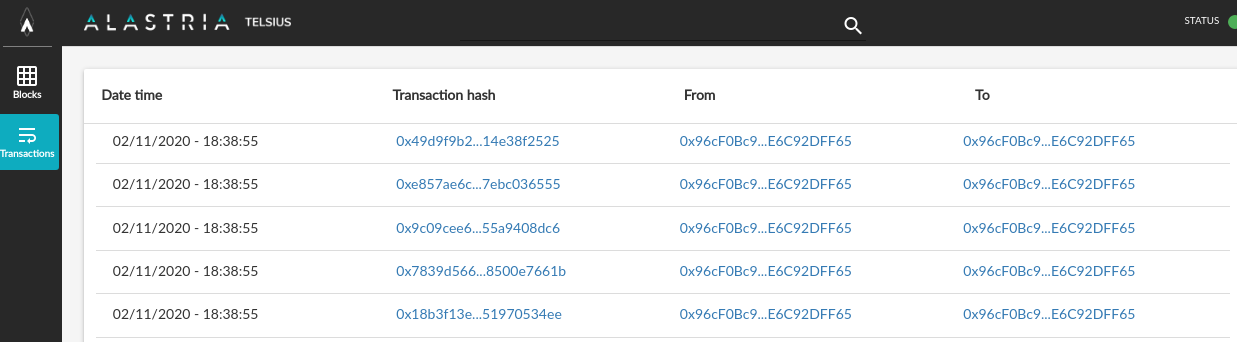
\includegraphics[width=1.1\textwidth]{Alastria-block-exporer.png}
                \caption{Alastria's Block explorer}
                \label{fig:alastria_block_explorer}
            \end{figure}
            \item \textbf{Immutability}. This property ensures that once something has been entered into the blockchain, it cannot be tampered or modified.
        \end{itemize}
        
        \subsubsection{How does Blockchain work?}
            A Blockchain is a growing list of records, called blocks (figure \ref{fig:linked_blocks}), that are linked using cryptography. Each block contains a hash of the previous block, the timestamp and a batch of valid transaction hashes encoded into a Merkle tree. The linked blocks form a chain. This iterative process confirms the integrity of the previous block, all the way back to the original genesis block (the first block of the network).
            \begin{figure}[h]
                \centering
                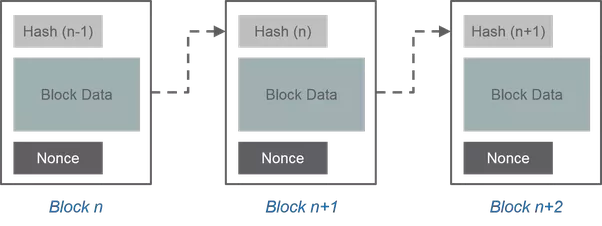
\includegraphics[width=1.0\textwidth]{block-example.png}
                \caption{Visual example of linked blocks}
                \label{fig:linked_blocks}
            \end{figure}
            
        \subsubsection{Types of blockchains}
            There are different kinds of Blockchain networks, each one with different features (figure  \ref{fig:blockchain_classification}). One of the most common classification is according to the architecture. The following figure shows a table with the classification.
            \begin{figure}[h]
                \centering
                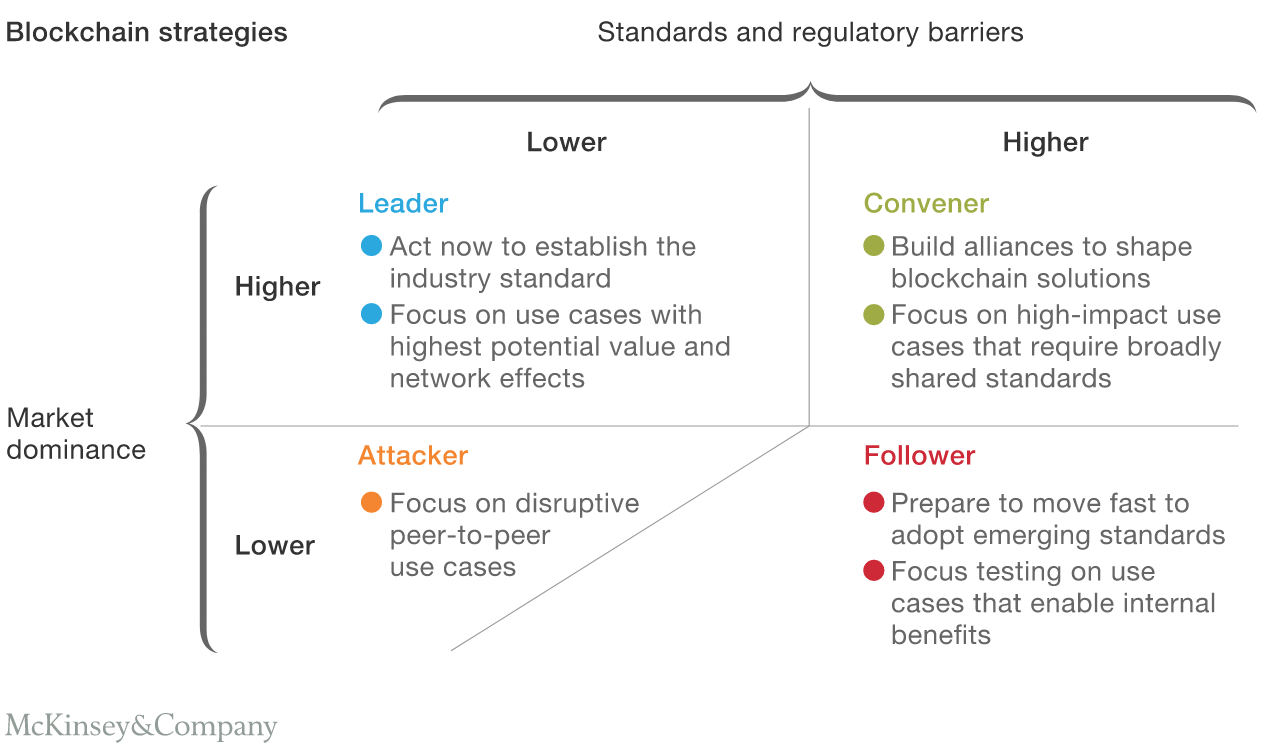
\includegraphics[width=1.0\textwidth]{Blockchain-types.png}
                \caption{Blockchain architecture classification by \textit{McKinsey\&Company}}
                \label{fig:blockchain_classification}
            \end{figure}

            \begin{itemize}
                \item \textbf{Public}. A public network is the one where everyone can join. Some examples of public networks are Bitcoin, Ethereum and Litecoin.
                \item \textbf{Private}. A private network is the one where only authorized members can join. Some examples of private networks are Quorum and Monax.
                \item \textbf{Permissionless}. A permissionless network is a private or public blockchain where every member can read and write.
                \item \textbf{Permissioned}. A permissioned network is a private or public blockchain where every member can read but only some can write. Some examples of public permissioned networks are Alastria and LACChain.
            \end{itemize}          
            Also, there are two more types of blockchain networks on the rise.
            \begin{itemize}
                \item \textbf{Consortium} or \textbf{hybrid networks}. These networks are private and permissioned, operated by known entities such as stakeholders of a given industry regrouped in a consortium or exploiting a shared platform. Some known examples are \textit{Hyperledger} \textit{Fabric}, \textit{R3 Corda} and \textit{Multichain}.
                \item \textbf{\acrfull{baas}}. These are cloud platforms hosted by a service provider to deploy blockchain applications. The service provider manages the blockchain network while the customer defines the business logic. Some of the examples are \textit{\acrfull{aws}} and \textit{Oracle} blockchain platforms.
            \end{itemize}
            
            \subsubsection{Uses of blockchain}
                With the different properties of blockchain technology, and the different types of networks, there are a lot of use cases (figure \ref{fig:blockchain_uses}). The best known use case is using the blockchain as a payment infrastructure, the best example is Bitcoin. But there are a lot of other use cases shown in the next figure.\\
                \begin{figure}[h]
                    \centering
                    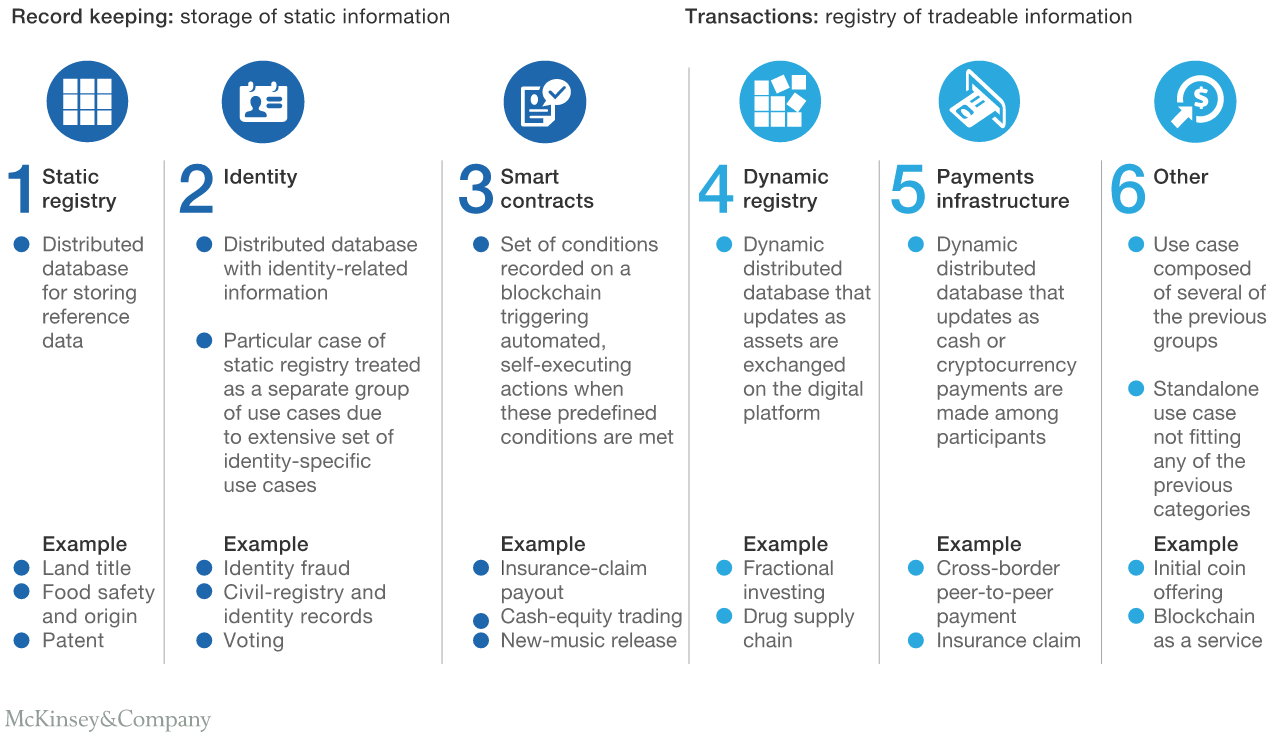
\includegraphics[width=0.95\textwidth]{Blockchain-uses.png}
                    \caption{Blockchain use cases table by \textit{McKinsey\&Company}}
                    \label{fig:blockchain_uses}
                \end{figure}
                
                In this document we are going to focus on the \acrfull{ssi} using blockchain.

    \subsection{Ethereum}
        Ethereum\cite{ethereum} (figure \ref{fig:ethereum_logo}) is an open-source, public, blockchain-based distributed ledger featuring smart contract functionality. It enables developers to build blockchain applications with business logic that execute in a trustless environment, while leveraging the high availability of the Ethereum network. 
        \begin{figure}[h]
            \centering
            
\includegraphics[width=0.5\textwidth]{ethereum-logo-portrait-purple.png}
            \caption{Ethereum logo}
            \label{fig:ethereum_logo}
        \end{figure}
        The principles behind Ethereum philosophy are\cite{ethereumWhitepaper}:
        \begin{itemize}
            \item \textbf{Simplicity}. The Ethereum protocol should be as simple as possible.
            \item \textbf{Universality}. Ethereum provides an internal Turing-complete scripting language. This language can be used to construct any logic, and any business case.
            \item \textbf{Modularity}. The Ethereum protocol is designed to be as modular as possible, to allow if one was to make a small protocol modification in one place, the application stack would continue to function as normally. 
            \item \textbf{Agility}. The protocol can be modified.
            \item \textbf{Non-discrimination} and \textbf{non-censorship}. The protocol should not restrict any usage.
        \end{itemize}
        
        \subsubsection{Ether}
            \acrfull{eth} is the native cryptocurrency used on the Ethereum network and is used to compensate miners who secure transactions. It is used to pay for gas, a unit of computation used in transactions and other state transitions.
            \acrlong{eth} also has many current use cases, such as a store of value, a medium of exchange, and a unit of account.
            
        \subsubsection{Ethereum Accounts}
            An Ethereum account or simply an “account” is the combination of an Ethereum address and it’s private key. An account can hold balance (\acrlong{eth}) and can send transactions. In Ethereum there are 2 types of accounts.
            \begin{itemize}
                \item \textbf{\acrfull{eoa}}. These accounts are a combination of public address and private key. This accounts:
                \begin{itemize}
                    \item Has an \acrlong{eth} balance
                    \item Can send transactions to Smart Contracts
                    \item Can send and receive \acrlong{eth} to/from another account
                    \item Is controlled by private keys
                    \item Has no associated code
                \end{itemize}
                \item \textbf{Contract accounts}: These accounts don’t have a corresponding private key. These accounts are generated when a Smart Contract is deployed in the blockchain. They are normally called “contracts” instead of contract accounts. A contract:
                \begin{itemize}
                    \item Has an \acrlong{eth} balance
                    \item They can receive \acrlong{eth} just like \acrshort{eoa}
                    \item Has associated code
                    \item Code execution is triggered by transactions or calls received from other contracts or accounts
                    \item When executed can manipulate its own persistent storage
                \end{itemize}
            \end{itemize}
        
        \subsubsection{Ethereum wallet}
            Wallets are software that are used to store and manage Ethereum accounts. Wallets allow the user to manage multiple accounts, provide functionality to sign transactions, track balances and so on. Wallets can be classified into two types.
            \begin{itemize}
                \item \textbf{Non-deterministic} wallet. These wallets use a random private key and generate a private key from it.
                \item \textbf{Deterministic} wallet. In this wallet, keys are derived from a seed. The seed allows a user to easily back up and restore a wallet without needing any other information, and in some cases allow the creation of public addresses without the knowledge of the private key.
            \end{itemize}
        
        \subsubsection{Ethereum stack}
            Like any software stack, the complete "Ethereum stack"\cite{ethereumStack} will vary from project to project depending on your business goals. However, the typical layers are:
            \paragraph{Ethereum Virtual Machine (EVM)}
                The \acrlong{evm}\cite{evm}, normally known as \acrshort{evm} is a software designed to emulate a machine with certain capabilities that make the Ethereum blockchain possible. We can program instructions for the \acrshort{evm}, using a series of opcodes, which we can then compile and translate into a specific bytecode or language that the \acrshort{evm} can understand and execute.\\
                
                The opcodes perform standard stack operations like \textit{XORAND}, \textit{ADD}, \textit{SUB}, etc. The \acrshort{evm} also implements a number of blockchain-specific stack operations, such as \textit{ADDRESS}, \textit{BALANCE}, \textit{SHA3}, \textit{BLOCKHASH}, etc. More specific information can be found at the official documentation\cite{opcodes}.\\
                
                To make programming easier for the virtual machine, a specialized high-level language called Solidity was created. This programming language is used to create Smart Contracts. Solidity first transforms opcodes and then these to bytecode. This bytecode is finally executed by the \acrshort{evm} to perform the specified operations of a  Smart Contract. All this means that the \acrshort{evm} can function as a real computer, executing from the simplest to the most complex operations.\\
                
                In the following sections we will talk in detail about the Smart Contracts and Solidity.
                
            \paragraph{EVM Characteristics}
                The \acrshort{evm} has a series of unique characteristics\cite{ethereumGavin}\cite{ethereumDocu}:
                \begin{itemize}
                    \item It provides a \textbf{high level of security}. As it is a virtual machine limited in the instructions (opcodes) and the way they are executed, \acrshort{evm} is capable of executing unreliable codes without disastrous consequences.
                    \item The \acrshort{evm} is a \textbf{completely decentralized} build. Each node within the Ethereum network runs a copy of the virtual machine and is synchronized with the rest of the nodes that make up the network. This guarantees that the instructions given by the \acrshort{evm} are executed as long as there is at least one active node. This allows access to the system from anywhere in the world, resisting censorship and guaranteeing access to network resources. Furthermore, it does not require the participation of third parties, and resources can’t be modified or altered.
                    \item Applications can be executed on the same blockchain network, without affecting other operations.
                    \item \acrshort{evm} is able to follow the “rules” of Smart Contracts.
                    \item The \acrshort{evm} has the ability to execute a series of well-defined opcodes.
                \end{itemize}
                
            \paragraph{How does it work?}
                The figure \ref{fig:blockchain_stack} defines how the \acrshort{evm} works\cite{queEsEvm}.
                \begin{figure}[h]
                    \centering
                    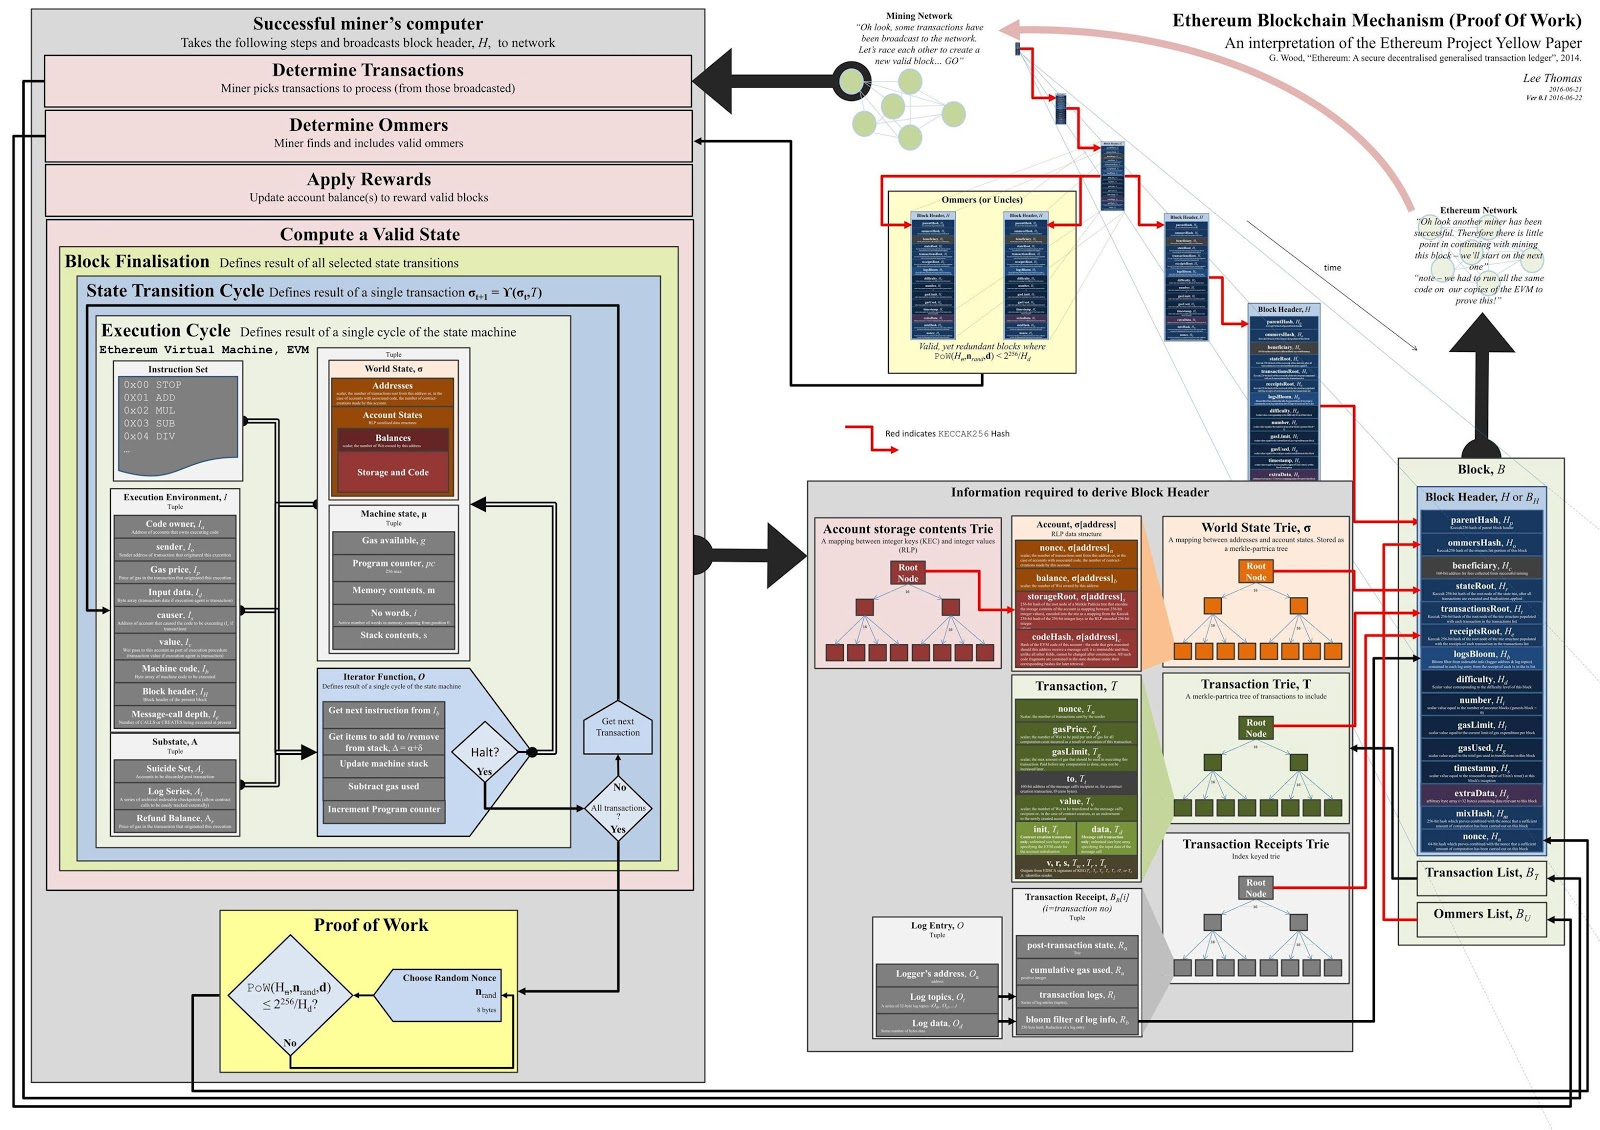
\includegraphics[width=1\textwidth]{evm-stack.jpeg}
                    \caption{\acrshort{evm} stack schema}
                    \label{fig:blockchain_stack}
                \end{figure}

                The Smart Contracts made with Solidity are compiled and converted to opcodes. These opcodes are transformed to bytecode, so it does facilitate the performance of the \acrshort{evm} tasks.\\

                Thus, each transaction and operation that is carried out on the Ethereum blockchain goes through this process, and its execution is carried out by the \acrshort{evm}, which at the end records everything on the Ethereum blockchain, leaving a public record of those operations. 

        \subsubsection{Smart Contracts}
            Sam Richards\cite{smartContracts}, a Software Engineer working on Ethereum defines the Smart Contract as 
            \begin{quote}
                \textit{a snippet of code that runs on the Ethereum blockchain. It's a collection of functions and data that resides at a specific address on the Ethereum blockchain.}

                \textit{Smart contracts are a type of Ethereum account. This means they have a balance and they can send transactions over the network. However they're not controlled by a user, instead they are deployed to the network and run as programmed. User accounts can then interact with a smart contract by submitting transactions that execute a function defined on the smart contract. Smart contracts can define rules, like a regular contract, and automatically enforce them via the code.}
            \end{quote}

        \subsubsection{Solidity}
            \begin{figure}[h]
                \centering
                
\includegraphics[width=0.4\textwidth]{solidity-logo.jpg}
                \caption{Solidity logo}
                \label{fig:solidity_logo}
            \end{figure}
            
            Solidity (figure \ref{fig:solidity_logo}) defines itself as an object-oriented, high-level language for implementing Smart Contracts. Smart Contracts are programs which govern the behaviour of accounts within the Ethereum state.\\
            
            Solidity\cite{solidityGit} was influenced by \textit{C++}, \textit{Python} and \textit{JavaScript} and is designed to target the \acrfull{evm}. Solidity is statically typed, supports inheritance, libraries and complex user-defined types among other features.\\

            Below is an example of a Smart Contract\footnote{Source code from \url{https://github.com/alastria/alastria-identity/blob/master/contracts/identityManager/AlastriaIdentityIssuer.sol}} written in Solidity\footnote{More details about Solidity can be found in the official documentation\cite{solidity}} (listing  \ref{lst:AlastriaIdentityIssuer}).
            
            \lstinputlisting[label={lst:AlastriaIdentityIssuer}, caption=Source code from AlastriaIdentityIssuer.sol, language=Solidity]{examples/alastriaSCs/identityManager/AlastriaIdentityIssuer.sol}

        \subsubsection{Ethereum Nodes}
            A Node refers to a piece of software which is an implementation of Ethereum that verifies all transactions in each block, keeping the network secure and the data accurate. They collectively store the state of the Ethereum blockchain and reach consensus on transactions to mutate the blockchain state.\\
            
            There are three types of nodes.
            \begin{itemize}
                \item \textbf{Full node}. These types of nodes store full blockchain data, participate in block validation, verifies all blocks and states and serves the network and provides data on request. Also, all states can be derived from a full node.
                \item \textbf{Light node}. Stores the header chain and requests everything else. Can verify the validity of the data against the state roots in the block headers and it is useful for low capacity devices, such as embedded devices or mobile phones, which can't afford to store gigabytes of blockchain data.
                \item \textbf{Archive node}. Stores everything kept in the full node and builds an archive of historical states. These nodes can be handy for services like block explorers, wallet vendors, and chain analytics.
            \end{itemize}
            By connecting your application to an Ethereum node via \acrshort{json} \acrshort{rpc}, your application is able to read data from the blockchain as well as broadcast new transactions to the network.

        \subsubsection{Ethereum Client APIs}
            While APIs are not a necessary piece of the stack, they abstract away much of the complexity of interacting directly with Ethereum nodes and Smart contracts.\\
            
            Most of these APIs are open source and maintained by the Ethereum community.

        \subsubsection{End User Applications}
            The final part of the stack is the user-facing applications, primarily web and mobile apps.  They are made for users so they do not need to know the application they're using is built using a blockchain. Also the end user applications are made to hide the complexity from the user.
            
        \subsubsection{Ethereum 2.0 (Eth2)}
            \acrshort{eth2}\cite{eth2} is a long-planned upgrade to the Ethereum network, it will reduce energy consumption, allow the network to process more transactions, and increase security.  Ethereum will become a proof-of-stake blockchain and introduce shard chains. Shard chains are like parallel blockchains that sit within Ethereum and take on a portion of the network's processing work.\\
            
            The phase 1 of Ethereum 2.0 is supposed to happen in 2021. The roadmap can be checked in the official website\cite{eth2Roadmap}.
            

    \subsection{JSON-RPC}
        JSON-RPC is a \acrfull{rpc} encoded in \acrshort{json}. It is a simple protocol that defines only a few data types and commands. JSON-RPC allows for notifications (data sent to the server that does not require a response) and for multiple asynchronous calls. It uses \acrshort{json} \textit{RFC-4627}\cite{rfc4627} as data format.\\
        
        The first officially released specification was \textit{JSON-RPC 1.0}\cite{json-rpc-1} published in 2005, but the last official specification is \textit{JSON-RPC 2.0}\cite{json-rpc-2} published in 2010 with several improvements.
        
        \subsubsection{JSON}
            \acrlong{json} mostly known as \acrshort{json} is a lightweight data-interchange format. It is human readable and easy to write. Also, it is easy for machines to parse and generate. It is based on a subset of the JavaScript Programming Language Standard ECMA-262 3rd Edition - December 1999. \acrshort{json} is a text format that is completely language independent but uses conventions that are familiar to several languages such as \textit{C}, \textit{C++}, \textit{Java}, \textit{JavaScript}, \textit{Perl}, \textit{Python} and many others.\\
                        
            \acrshort{json} is built on two structures\cite{jsonSchema}:
            \begin{itemize}
                \item A collection of name-value pairs (figure \ref{fig:json_objects}). In various languages, this is realized as an Object, Record, Struct, Dictionary, ...
                \begin{figure}[h]
                    \centering
                    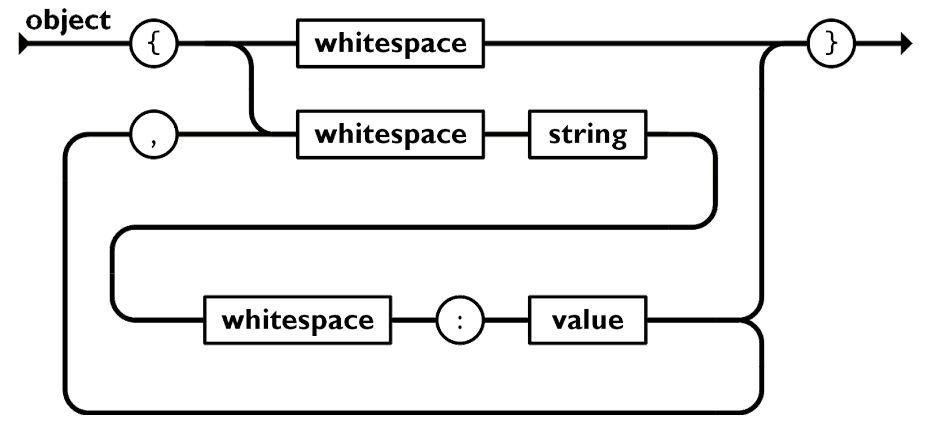
\includegraphics[width=0.6\textwidth]{json-objects.png}
                    \caption{\acrshort{json} objects schema}
                    \label{fig:json_objects}
                \end{figure}
                \item An ordered list of values (figure \ref{fig:json_arrays}). In most languages, this is realized as an Array, Vector, List, ...
                \begin{figure}[h]
                    \centering
                    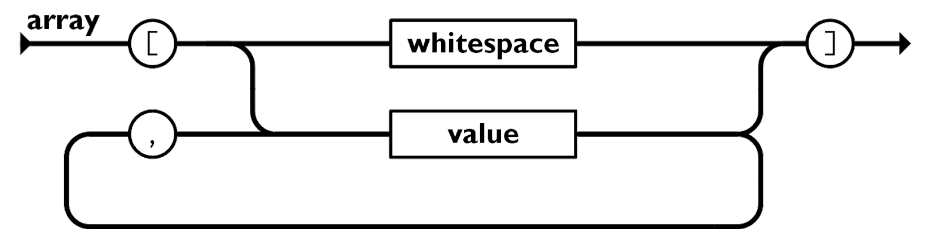
\includegraphics[width=0.6\textwidth]{json-arrays.png}
                    \caption{\acrshort{json} array schema}
                    \label{fig:json_arrays}
                \end{figure}
            \end{itemize}

        \subsubsection{RPC}
            A \acrfull{rpc}\cite{rpc} is when a computer program causes a procedure to execute in a different address space (commonly on another computer), which is coded as if it were a local procedure call. That is, the programmer writes essentially the same code whether the program will run locally or in a remote machine.\\
            
            The transparency is one of the great strengths of \acrshort{rpc}, because the application software does not contain any communication code, it is independent of:
            \begin{itemize}
                \item The communication hardware and protocols used
                \item The operative system
                \item The calling sequence needed to use the communication software layer
            \end{itemize}
            
            \paragraph{How RPC works}
                From the point of view of a remote call, the calling program is known as client, and the subroutine it calls is known as the server\cite{rpcInOS}\cite{howRPC}. When the client calls the server, the \acrshort{rpc} system must take care of:
                \begin{itemize}
                    \item Taking all the parameters which are passed to the subroutine and transferring them to the remote node
                    \item Having the subroutine executed on the remote node
                    \item Transferring back all the parameters which are returned to the calling routine
                \end{itemize}
                
                In the next figure (figure \ref{fig:rpc_schema}) we can see the typical \acrshort{rpc} communication schema.
                \begin{figure}[h]
                    \centering
                    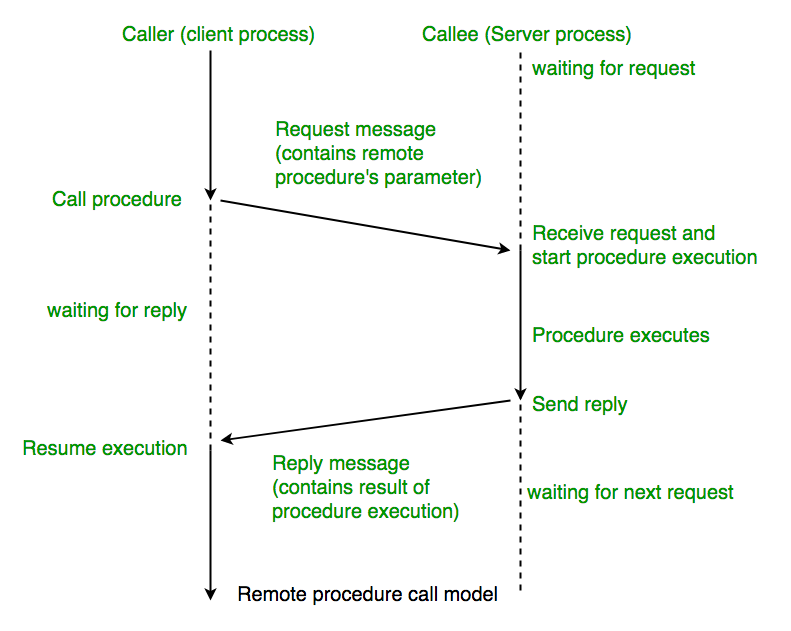
\includegraphics[width=0.7\textwidth]{rpc.png}
                    \caption{\acrshort{rpc} schema}
                    \label{fig:rpc_schema}
                \end{figure}
                The most common method of doing this is by the use of stub modules (figure \ref{fig:rpc_mechanism}). The client is linked to a client stub module. This is a subroutine which looks like the remote subroutine, but on the inside, it is almost empty. All it does is take the values of the parameters which are passed to it, and put them in a message. This is known as marshalling.\\

                The client stub then uses a routine in the \acrshort{rpc} \acrfull{rts} to send the message off and wait for a reply message. When the reply arrives, the stub unmarshals the parameters that were returned in the reply message, putting their values into the variables of the calling program. The client stub then returns to the calling program just like a normal subroutine.\\

                The server stub (located in the remote machine) is called by the \acrshort{rpc} \acrshort{rts} when the message arrives from the client. The server stub performs the unmarshall of the parameters passed to the subroutine, calling the subroutine, and marshalling the return parameters. 
                \begin{figure}[h]
                    \centering
                    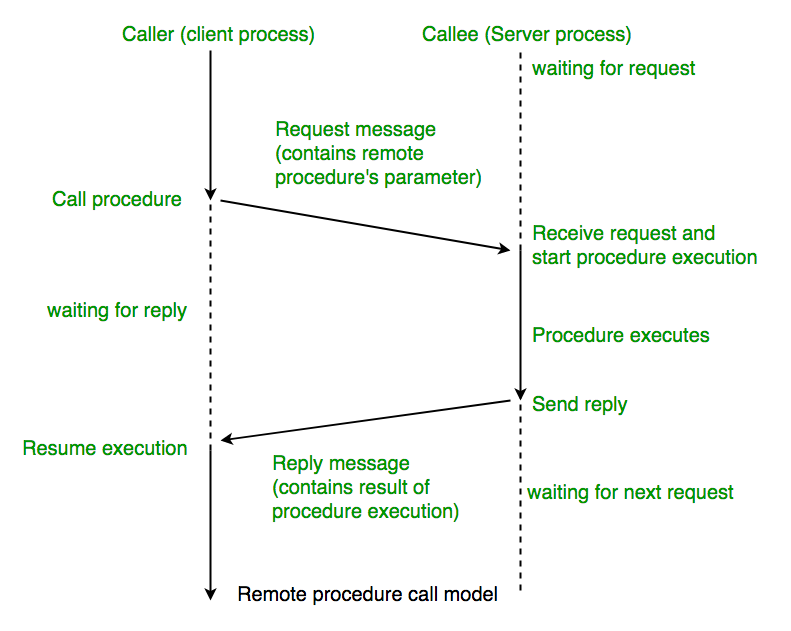
\includegraphics[width=0.7\textwidth]{rpc-mecha.png}
                    \caption{\acrshort{rpc} mechanism}
                    \label{fig:rpc_mechanism}
                \end{figure}
                All the communication details are handled by the \acrshort{rpc} \acrshort{rts}, so the stubs contain only the code which is specific to the application involved\cite{rpc2}.
                \begin{itemize}
                    \item In order to produce stub modules, it is need to know
                    \item The names of the procedures in the package (set of procedures)
                    \item The number of parameters which they take
                    \item The data type of each parameter
                    \item The direction in which each parameter is transferred
                \end{itemize}
        \subsubsection{JSON-RPC 1.0}
            The general mechanism consists of two peers establishing a data connection\cite{json-rpc-1}. Peers may invoke methods provided by the older peer. To invoke a remote method, a request serialized using \acrshort{json} is sent. The request is a single \acrshort{json} Object with three properties: 
            \begin{itemize}
                \item \textbf{method}: The name of the invoked method.
                \item \textbf{params}: The params passed as arguments to the method. It is an Array of Objects.
                \item \textbf{id}: The request id. It can be of any type. It is used to match the response with the reply. If it is a notification request, it must be Null.
            \end{itemize}
            The request must be replied unless it is a notification (does not need a response). The response is also a single Object serialized using \acrshort{json} and has this properties:
            \begin{itemize}
                \item \textbf{result}: The Object returned by the invoked method. It is Null in case there was an error.
                \item \textbf{error}: An error Object if there was an error while invoking the method. It is Null if there was no error.
                \item \textbf{id}: The id of the request that was sent. 
            \end{itemize}
            JSON-RPC does not require a certain transport protocol, but \acrshort{tcp}/IP socket streams are encouraged. The request and the response are sent to the peers through byte streams.\\

            Also \acrshort{http} can be used as the communication transport. The request must be sent as an \textit{\acrshort{http} POST} with all the serialized Objects. Once the client has received the response, it must reply with another \textit{\acrshort{http} POST}. A non-valid request will result in closing the connection.
        \subsubsection{JSON-RPC 2.0}
            This specification\cite{json-rpc-2} works almost the same way as the JSON-RPC 1.0 but it has several upgrades.\\
            
            The request Object has the following properties:
            \begin{itemize}
                \item \textbf{jsonrpc}: The version of the JSON-RPC protocol. It must be exactly “2.0”.
                \item \textbf{method}: A String containing the name of the method.
                \item \textbf{params}: A Structured value (Object or Array) with the parameter values passed as arguments to the method.
                \item \textbf{id}: It is a String, Number or \textit{Null} identifier. If it is not included, it is assumed to be a notification. Normally it should not be \textit{Null} because this specification uses a value of \textit{Null} for responses with unknown id. Also, JSON-RPC 1.0 uses \textit{Null} for notifications, and it causes confusion in handling.
            \end{itemize}
            Similarly, the response from the server is expressed as a single \acrshort{json} Object with the following properties:
            \begin{itemize}
                \item \textbf{jsonrpc}: As in the request, it must exactly be “2.0”
                \item \textbf{result}: It is required on success, but must not exist if there was an error.
                \item \textbf{error}: It is required on error, but must not exist if there was no error. It must be an Object with the following properties:
                \begin{itemize}
                    \item \textbf{code}: A Number that indicates the error type occurred.
                    \item \textbf{message}: The provided short description of the error.
                    \item \textbf{data}: A Primitive (String, Number, Boolean or Null) or Structured (Object or Array) with additional information about the error. This may be omitted and it is defined by the server. The error codes are nearly the same as those suggested for XML-RPC\cite{rpc-err}.
                \end{itemize}
                \item \textbf{id}: This property must be the same as the value of the requested Object. If there was an error, it must be \textit{Null}.
            \end{itemize}
            To send several requests at the same time, the client may send an Array with all the request objects. It is called batch. The response from the server should be another Array containing the response objects after all the requests have been processed. The server may process the batch as a set of concurrent tasks. Also, the response objects may be returned in any order within the Array. Thanks to the id server and client will match the context between requests and responses.
            
        \subsection{JSON Web Tokens}
            In the RFC-7519\cite{rcf-jwt}, the \acrfull{jwt} is defined as:
            \begin{quote}
                \textit{\acrfull{jwt} is a compact claims representation format intended for space constrained environments such as \acrshort{http} Authorization headers and URI query parameters.  \acrfull{jwt}s encode claims to be transmitted as a \acrshort{json} object that is used as the payload of a \acrfull{jws} structure or as the plaintext of a \acrfull{jwe} structure, enabling the claims to be digitally signed or integrity protected with a \acrfull{mac} and/or encrypted. \acrshort{jwt}s are always represented using the \acrshort{jws} Compact Serialization or the \acrshort{jwe} Compact Serialization.} 
           \end{quote}
          
          Basically a \acrshort{jwt} is a \acrshort{json} that has three parts:
          \begin{itemize}
              \item \textbf{Header}: provides important information about the token.
              \item \textbf{Payload}: it contains the actual information that will be transmitted to the application. The information is provided as key-value pairs. The keys are called claims.
              \item \textbf{Signature}: It is created using the Base64 encoding of the header and payload, as well as the specified signing or encryption method. The structure is defined by \acrfull{jws}.
          \end{itemize}
          Below (figure \ref{fig:jwt-ex}) we can see an example of signed and unsigned \acrshort{jwt}.
          \begin{figure}[h]
                \centering
                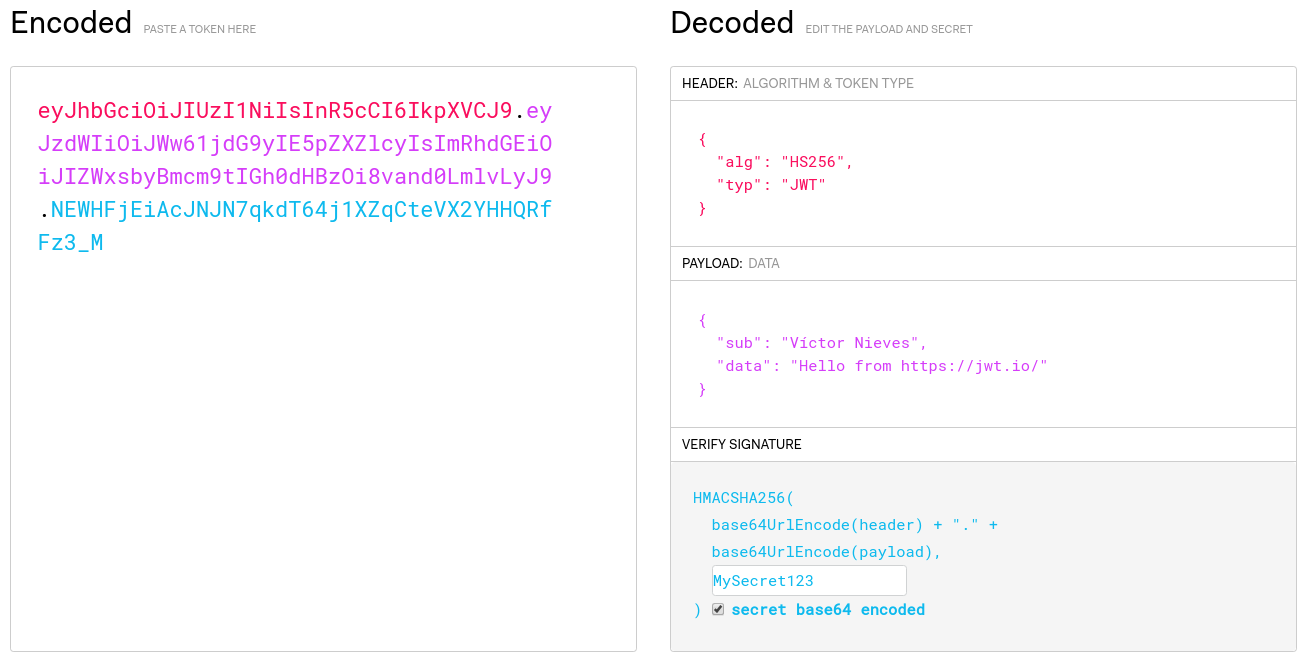
\includegraphics[width=1\textwidth]{jwt-example.png}
                \caption{Example of signed and unsigned \acrshort{jwt}}
                \label{fig:jwt-ex}
          \end{figure}

        
        \subsection{Self-Sovereign Identity}
            The idea of the \acrlong{ssi} was born to solve the problems with the current physical and digital identifications.\\
            Some of the physical IDs problems are:
            \begin{itemize}
                \item The process of obtaining them is time consuming, bureaucratic and costly. For both the ID Owner and Issuer Organization. 
                \item If you lose your ID and need to obtain a new one.
                \item Physical IDs can be defrauded with impersonation and ID theft. The only way to check its authenticity is often by contacting the issuing organization.
                \item They are not private.
            \end{itemize}
            Also, some problems with the current digital IDs are:
            \begin{itemize}
                \item Having to register and sign up with different login credentials to every new online service is uncomfortable for the user. 
                \item Tedious on-boardings.
                \item Managing multiple passwords is hard and using the same password is a security risk.
                \item The user has no control over what data is being shared and with whom.
                \item The verification of your credentials is dependent on the availability of the issuer.
                \item Third party login services have a financial incentive to collect and store your data.
                \item The user's personal data is stored on the issuer’s servers. Centralized storages of personal data create \textit{“honeypots”}. This data is at risk of breaches, leaks or hacks.
            \end{itemize}

            \acrfull{ssi} is a digital identification scheme in which the user acquires the responsibility of managing how and in what quantity their personal data is used. To do this, it allows the creation of digital \textit{“identity cards}” that can be general for any service or specific for each case. \\
            The main characteristics of \acrlong{ssi} are\cite{ssi-guide}:
            \begin{itemize}
                \item It is secure and digital peer-to-peer channel is established between Issuer, owner and Verifier.
                \item When credentials are exchanged not even the \acrlong{ssi} system provider knows what is being exchanged.
                \item Credentials are tamper-proof through the use of cryptography.
                \item They are private and under the owner control. \acrshort{ssi} uses Selective Identity disclosure technology.
                \item The Owner chooses what data they want to “show” and is always in control of the relationship with ID Verifiers.
                \item Credentials can be verified anywhere, at any time.
                \item Personal Data is not stored on centralized servers.
                \item \acrshort{ssi} tries to abolish multiple passwords. You just need to know your wallet password.
            \end{itemize}

            \subsubsection{How does it work?}
                In order to explain how the \acrshort{ssi} works, we have to see some concepts previously.
                \paragraph{Actors}
                    The figure \ref{fig:trust-triangle} explains the different actors\cite{ssi-guide} that take place in the process.
                    \begin{figure}[h]
                        \centering
                        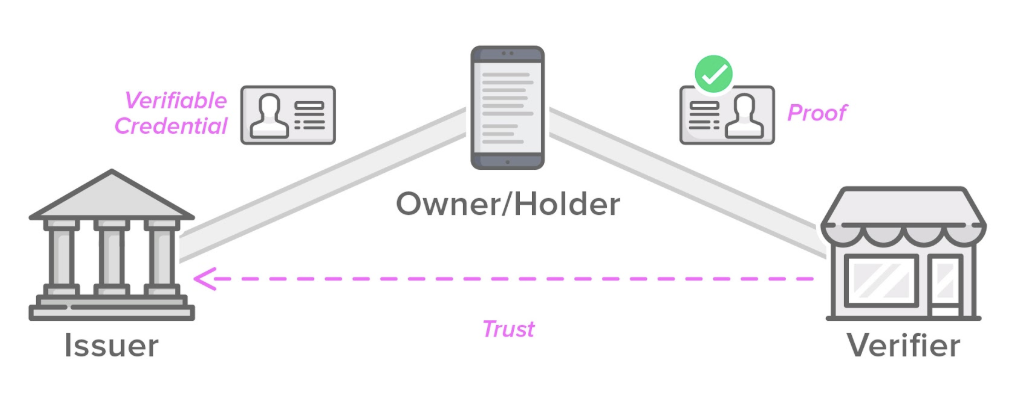
\includegraphics[width=0.7\textwidth]{trust-triangle.png}
                        \caption{Trust triangle / Actors in \acrshort{ssi}}
                        \label{fig:trust-triangle}
                    \end{figure}
                    \begin{itemize}
                        \item \textbf{Owner / Holder}: orders the creation of credentials. He stores the credentials locally. He has the power to revoke access to these credentials.
                        \item \textbf{Issuer}: provides a digital service. It needs to identify users. Does not need to store user data.
                        \item \textbf{Verifier}: creates the credentials with the data provided by the user. It does not store user data (although it has access to it at the time of creation of the credential).
                    \end{itemize}
            
                \paragraph{Verifiable Credentials}
                    According to the World Wide Web Consortium \textit{\acrshort{w3c}}\cite{w3c-vc}\footnote{\label{footnote-w3c}More information about Verifiable Credentials and Verifiable Presentations can be found in the main web page of \acrshort{w3c}\cite{w3c-vc}}:
                    \begin{quote}
                        \textit{A verifiable credential can represent all of the same information that a physical credential represents. The addition of technologies, such as digital signatures, makes verifiable credentials more tamper-evident and more trustworthy than their physical counterparts.}
                    \end{quote}
                    In the figure \ref{fig:ssi-vc}, we can see clearly the relationship between Issuer, Holder and Verifier and how a Verifiable Data Registry (normally a blockchain) is used to verify the credentials’ data without the need to contact the issuing party.
                    \begin{figure}[h]
                        \centering
                        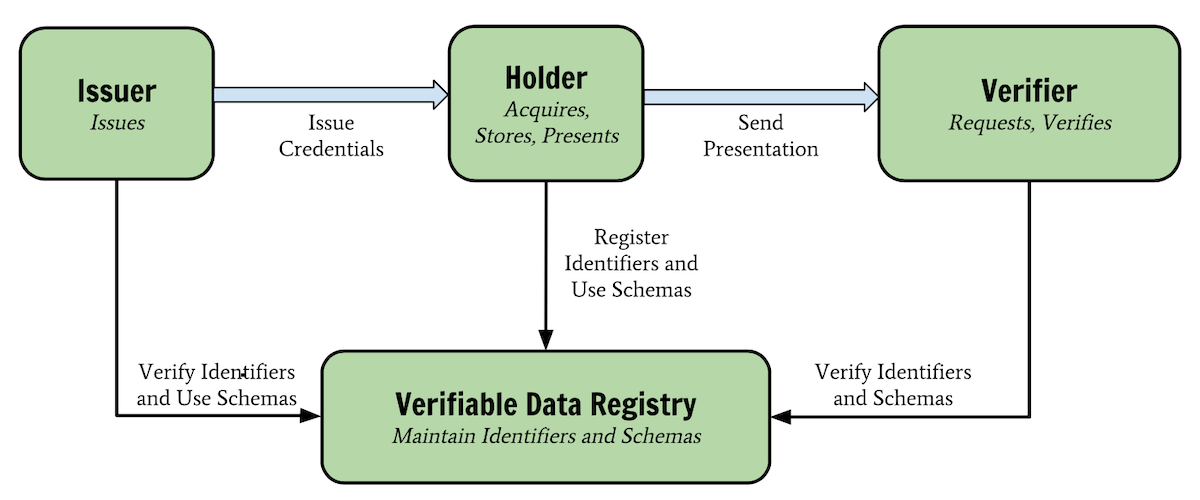
\includegraphics[width=1.0\textwidth]{ssi-vc.png}
                        \caption{The roles and information in a \acrshort{ssi} ecosystem by \acrshort{w3c}}
                        \label{fig:ssi-vc}
                    \end{figure}
                
                \paragraph{Verifiable Presentations}
                    According to \acrshort{w3c}\cite{w3c-vc}\footref{footnote-w3c}:
                    \begin{quote}
                        \textit{A verifiable presentation expresses data from one or more verifiable credentials, and is packaged in such a way that the authorship of the data is verifiable. If verifiable credentials are presented directly, they become verifiable presentations. Data formats derived from verifiable credentials that are cryptographically verifiable, but do not of themselves contain verifiable credentials, might also be verifiable presentations.}
                        
                        \textit{The data in a presentation is often about the same subject, but might have been issued by multiple issuers. The aggregation of this information typically expresses an aspect of a person, organization, or entity.}
                    \end{quote}
                    In the figure \ref{fig:ssi-vp} we can see the components of a verifiable presentation.
                    \begin{figure}[ht] 
                        \centering
                        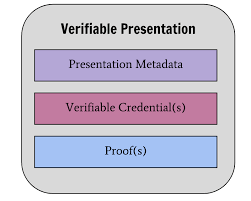
\includegraphics[width=0.5\textwidth]{ssi-vp.png}
                        \caption{Basic components of a verifiable presentation by \acrshort{w3c}}
                        \label{fig:ssi-vp}
                    \end{figure}
                \paragraph{Decentralized Identifiers (DIDs)}
                    According to \acrshort{w3c}\cite{w3c-did}\footnote{More information about the \acrshort{did}s can be found in the main web page of \acrshort{w3c}\cite{w3c-did}}:
                    \begin{quote}
                        \textit{\acrfull{did}s are a new type of identifier that enables verifiable, decentralized digital identity. A \acrshort{did} identifies any subject (e.g., a person, organization, thing, data model, abstract entity, etc.) that the controller of the \acrshort{did} decides that it identifies. In contrast to typical, federated identifiers, \acrshort{did}s have been designed so that they may be decoupled from centralized registries, identity providers, and certificate authorities. Specifically, while other parties might be used to help enable the discovery of information related to a \acrshort{did}, the design enables the controller of a \acrshort{did} to prove control over it without requiring permission from any other party. \acrshort{did}s are URIs that associate a \acrshort{did} subject with a \acrshort{did} document allowing trustable interactions associated with that subject.}
                        
                        \textit{Each \acrshort{did} document can express cryptographic material, verification methods, or service endpoints, which provide a set of mechanisms enabling a \acrshort{did} controller to prove control of the \acrshort{did}. Service endpoints enable trusted interactions associated with the \acrshort{did} subject. A \acrshort{did} document might contain the \acrshort{did} subject itself, if the \acrshort{did} subject is an information resource such as a data model.}
                    \end{quote}
                    
                \paragraph{Wallets}
                    A wallet\cite{ssi-wallets} is a private repository that allows its owner to store, manage, and present keys and identity credentials.\\
                    
                    Some of the properties every wallet should have are:
                    \begin{itemize}
                        \item Provide secure access to the owner.
                        \item Guarantee that only authorized entities can access to it.
                        \item Ensure security and data encryption.
                        \item Provide recovery for keys and credentials.
                        \item Be connected to the blockchain where the \acrshort{did} was registered.
                        \item Provide mechanism for subjects and issuers to change the status of their credentials.
                        \item Provide mechanism for the owner to erase all the data associated with them.
                    \end{itemize}
                    Normally, when we talk about wallet, we think in mobile wallets (mobile applications), but a wallet can also be in a desktop, browser, hardware or the cloud.
                
                \paragraph{Functioning}
                    In the architecture\cite{how-to-ssi} we find a credential provider (\textit{issuer}) that is responsible for signing the data provided by the user by creating a certificate. Then, it will be signed by the user, attesting that the certificate generated by the issuer does not contain missing or altered information.\\
                    
                    Signatures by both the user and the issuer are performed using DIDs, which are traditional asymmetric keys. The public key of both is stored publicly on the blockchain. In this way, later on, the service provider (\textit{verifier}) that wants to identify the user will only have to verify that the signatures are correct and that, therefore, the credential has not been altered and contains the same information that the user provided to the identity provider.\\
                    
                    In the next figure (figure \ref{fig:ssi-scheme}) we can see a graphic scheme of the explained above.
                    \begin{figure}[h]
                        \centering
                        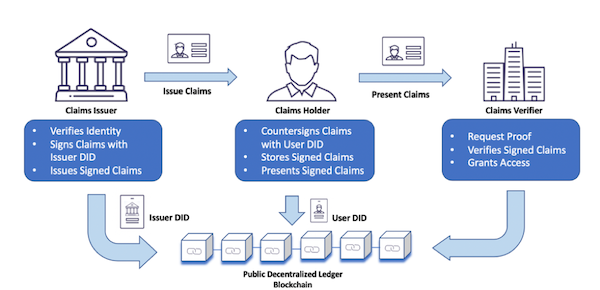
\includegraphics[width=1.0\textwidth]{how-to-ssi.png}
                        \caption{SSI functioning scheme}
                        \label{fig:ssi-scheme}
                    \end{figure}

            \subsubsection{Use cases}
                \acrlong{ssi} is benefiting several industries\cite{ssi-guide}, some examples are: streamlining bureaucratic procedures, improving a more efficient healthcare system, detecting academic and business fraud, creating a better user experience while onboardings or helping companies avoid personal data breaches and \acrshort{gdpr}\cite{gdpr} fines.

            \subsubsection{Alastria}
                Alastria (figure \ref{fig:alastria_logo}) is the world’s first nation-wide, multi-sectorial, enterprise grade, permissioned blockchain network. A non-profit association open to all types of companies and organizations with the mission to contribute to the creation of a diverse innovation ecosystem. Alastria is technology agnostic and offers the networks promoted by its partners as well as a user centric Digital Identity model, the Alastria ID, focused on ensuring the legal validity of the transactions on the networks.
                \begin{figure}[h]
                    \centering
                    
\includegraphics[width=0.5\textwidth]{alastria-logo.png}
                    \caption{Alastria logo}
                    \label{fig:alastria_logo}
                \end{figure}
                \paragraph{Alastria ID}
                    Alastria ID (figure \ref{fig:alastria_id_logo}) is a digital identity model proposed by the Consortium for use in digital services, even beyond blockchain technology itself and inspired by the Self Sovereign Identity concept.\\
                    \begin{figure}[h]
                        \centering
                        
\includegraphics[width=0.2\textwidth]{alastria-id-logo.png}
                        \caption{Alastria ID logo}
                        \label{fig:alastria_id_logo}
                    \end{figure}
                
                    The Identity Commission of Alastria ID\cite{alastria-context} has taken a further step in the typical functionalities of this tool. It has followed the recommendations of the ID of the \acrfull{w3c}\cite{w3c}, the international community that develops Internet standards. It has even been improved. Alastria ID has been developed in accordance with the demanding \acrfull{gdpr}\cite{gdpr} (General Data Protection Regulation), and \acrfull{eidas}\cite{eidas}..\\

                    The Alastria Standards Commission, which participates in all international and national standardization bodies, has collaborated in the process of the definition of the Alastria ID. The model specification inspired the Spanish identity standard UNE 71307\cite{une-71307} and the decentralized identity framework of EBSI\cite{ebsi} (European Blockchain Services Infrastructure), the blockchain of European public administrations.\\
                    
                    In the next section we will delve into the peculiarities and details of the different tools created by Alastria to facilitate the use of Alastria ID.

            \subsubsection{Other implementations}
                At present, \acrlong{ssi} is still at an early stage. However, there is already an extensive catalog of projects that show their potential. Different working groups and standardization agencies have been working to develop new standards and protocols that are the base of the \acrshort{ssi} model\cite{ssi-wallets}. Some of these groups are: the \textit{\acrfull{dif}}, the \textit{\acrfull{ebsi}}, the \textit{\acrfull{ietf}}, \textit{LACChain}, \textit{NIST}, \textit{Sovrin}, \textit{OASIS}, the \textit{\acrfull{oidf}}, and the \textit{\acrfull{w3c}}.\\
                
                There are also a few existing solutions on the market which leverage new standards and protocols for \acrshort{ssi}:
                \paragraph{Serto/uPort}
                    Serto\cite{serto} (figure \ref{fig:uport}) formerly known as uPort\cite{uport} is a web-based wallet and identity management system created by ConsenSys\cite{consenSys}. This project allows users (people) to manage their own private and public keys, without the need for intermediaries. It allows these keys to be recovered without the user having to lose their identity. The system consists of a mobile application (wallet), where the user can manage their identity, can receive and issue claims. A claim is nothing more than a data structure where \textit{"someone says something about another person"}. These claims make up the identity of the user, and can be displayed to identify themselves in front of entities. The identity is controlled by the user, without problems of someone questioning the legitimacy or altering the identity data.
                    \begin{figure}[h]
                        \centering
                        
\includegraphics[width=.2\textwidth]{serto-logo.png}\hfill
                        
\includegraphics[width=.2\textwidth]{uport-logo.png}\hfill
                        
\includegraphics[width=.3\textwidth]{consensys-horizontal-logo.png}
                        \caption{Serto, uPort and ConsenSys logos}
                        \label{fig:uport}
                    \end{figure}
                    
                \paragraph{David19}
                    David19\cite{david19} (figure \ref{fig:david19}) emerges as a collaborative application in which any citizen can participate to promote digital transformation in order to face health emergencies caused by the COVID-19 pandemic in 2019. This project created by LACChain\cite{lacchain} allows users (citizens) to share their information in solidarity, in a secure and anonymous way through self-claimed credentials. With this information, risk maps can be generated in real time, thus allowing authorities to make key decisions in managing the pandemic.\\
                    \begin{figure}[h]
                        \centering
                        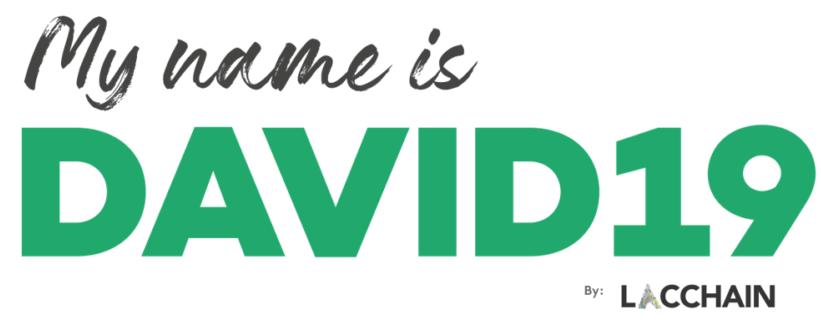
\includegraphics[width=.3\textwidth]{logo-david19.png}
                        \caption{David19 logo}
                        \label{fig:david19}
                    \end{figure}
                    
                    In a second phase\cite{que-es-david19}, it is proposed that the entities join the ecosystem, and that they can issue more sophisticated credentials, such as permits to return to work, medical certifications or academic degrees. The ultimate goal of David19 is for a person to only need a mobile device (wallet) to demonstrate that they are fit to get on a plane, return to work, visit a museum, etc., all in compliance with applicable regulations. The final objective of David19 is that a person only needs a mobile device (wallet) to demonstrate that they are healthy to get on a plane, return to work, visit a museum, etc., all in compliance with the regulations that apply at the time and the place.

                \paragraph{Hyperledger Indy}
                    Contributed by the Sovrin Foundation\cite{sovrin-yt}\cite{sovrin}, Hyperledger Indy\cite{indy-gh}\cite{indy} (figure \ref{fig:indy}) enables people to manage and control their digital identities. Rather than companies storing large amounts of personal data, what they store are indicators of identity. One of Hyperledger Indy's key tenets is its privacy-by-design approach: \textit{"it's not about protecting data but about designing so, that data doesn't need protection"}.\\
                    \begin{figure}[h]
                        \centering
                        
\includegraphics[width=.3\textwidth]{hyper-indy.png}
                        
\includegraphics[width=.3\textwidth]{Sovrin-Logo.jpg}\hfill
                        \caption{Hyperledger Indy and Sovrin logos}
                        \label{fig:indy}
                    \end{figure}
                    
                    The proposal is based on having multiple \acrshort{did}s for each user. Every time an agent is operated to give the user's credentials, a new \acrshort{did} will be generated.\\
                    
                There are also other solutions\cite{ssi-wallets} like \textit{Evernym}, \textit{KayTrust} (by Everis) and \textit{Rem} (by World Data).
\newpage

\section{Alastria ID}
    As we have seen, Alastria is a Spanish blockchain consortium, in which multiple companies and organizations are collaborating in different Github repositories\footnote{https://github.com/alastria}, promoting the implementation of a new digital identity model known as \acrlong{ssi}. In Alastria this implementation is called Alastria ID. Its mission is to reach all sectors and contribute to the creation of an innovation ecosystem that is as diverse as possible. \\
    
    \begin{figure}[h]
        \centering
        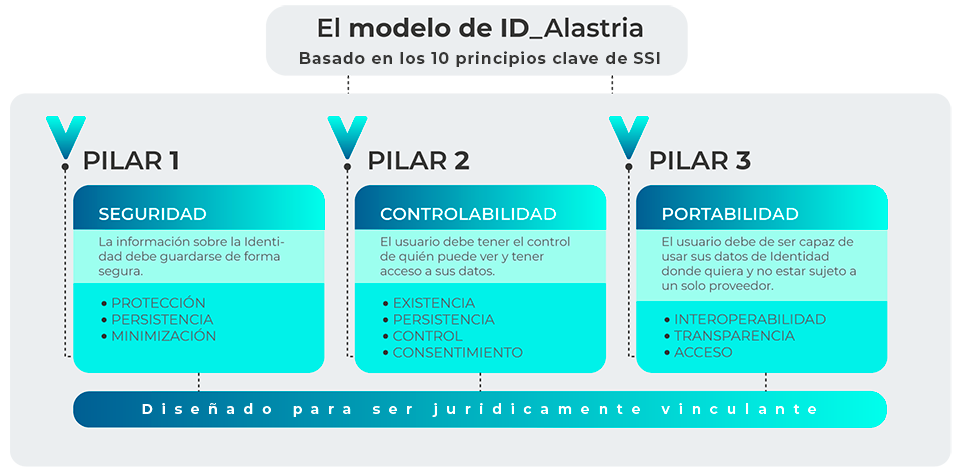
\includegraphics[width=1.0\textwidth]{pilares_alastria.png}
        \caption{Alastria ID model}
        \label{fig:pilares_alastria}
    \end{figure}
                    
    As the figure \ref{fig:pilares_alastria} obtained from the Alastria main website\footnote{https://alastria.io/en/id-alastria/} represents, the Alastria ID model is based in the 10 key principles of the \acrshort{ssi}. It is designed to be legally binding, and its three fundamental pillars are:
    \begin{itemize}
        \item \textbf{Security}: identity information must be kept secure. This means protection, persistence and minimization.
        \item \textbf{Controllability}: the user must have control of who can see and have access to their data. This means existence, persistence, control and consent.
        \item \textbf{Portability}: the user must be able to use their data wherever they want and not be subject to a single provider. This means interoperability, transparency and access.
    \end{itemize}
    
    \subsection{Actors}
        In the model several actors are defined, with different functionalities.
         \begin{itemize}
             \item \textbf{Entity}: Company or organization (legal person). An entity can be one or both:
             \begin{itemize}
                 \item \textbf{Service Provider}: Entity which requests information from a subject, so \textbf{it creates Presentation Requests and receives Presentations}.
                 \item \textbf{Issuer}: It can help anyone to create a new identity. Also this kind of entity can emits certified information about a subject, so \textbf{it creates Credentials}.
             \end{itemize}
             \item \textbf{Subject}: Person (natural or legal) who \textbf{has information certified by an Issuer and sends it to a Service Provider}, so it receives credentials and creates presentations. It is the information owner. This information is saved and controlled from a wallet.
             \item \textbf{Admin}: It is the \textbf{identity} (account) \textbf{that deployed the Smart Contracts}. \textbf{It is only used to create the first entity} (Issuer). \textbf{All other identities must be created by Issuers}.
        \end{itemize}
        In the next figure (\ref{fig:roles-ala}) we can see a visual explanation of the data flow between the different actors.
        \begin{figure}[h]
            \centering
            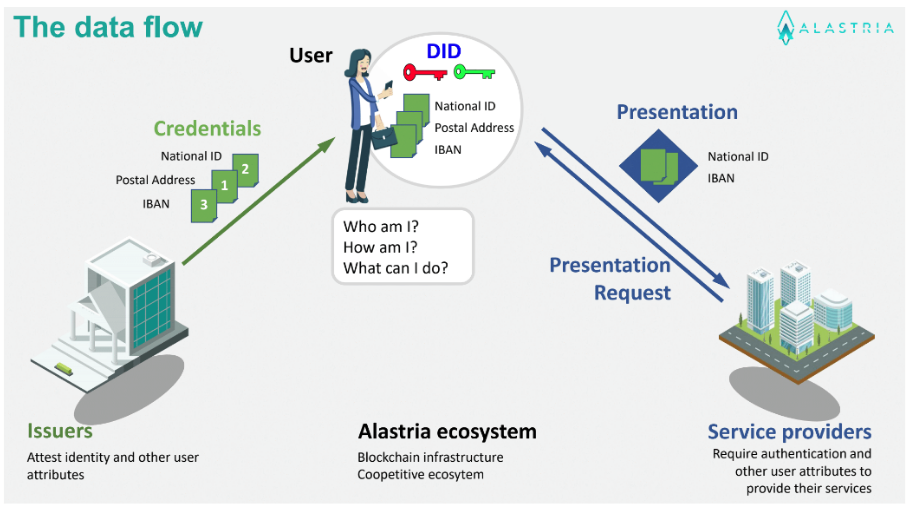
\includegraphics[width=1.0\textwidth]{roles-ala.png}
            \caption{Data flow between different actors in Alastria}
            \label{fig:roles-ala}
        \end{figure}

    \subsection{Alastria ID Specification}
        In this section we are going to see the different objects defined by Alastria for the model.
        \subsubsection{DIDs}
            As we have seen previously, the \acrfull{did}s are a type of identifier that allows the verification of decentralized identities. It should be noted that all entities, regardless of their role, have a \acrshort{did} that identifies them. At Alastria, the W3C standard is followed with a few minor differences.
            \begin{itemize}
                \item It will include the type of network in which the \acrshort{did} has been registered.
                \item It will also include the blockchain network and the network ID where the \acrshort{did} is registered.
            \end{itemize}
            
            Alastria \acrshort{did}s have the following format (listing \ref{lst:did_format}):
            \lstinputlisting[label={lst:did_format}, caption=\acrshort{did} format]{examples/codeSnippets/did_format.txt}
            Where:
            \begin{itemize}
                \item \textbf{"ala"}: specifies that this is a \acrshort{did} for Alastria.
                \item \textbf{"network"}: specifies the technology used on that network. 
                \item \textbf{"net-id"}: defines the specific Alastria blockchain network instance.
            \end{itemize}
            Possible examples of \acrshort{did}s are (listing \ref{lst:did_ex}):
            \lstinputlisting[label={lst:did_ex}, caption=Examples of \acrshort{did}s]{examples/codeSnippets/did_examples.txt}

        \subsubsection{Artifacts}
            Alastria Artifacts are currently coded as \acrshort{jwt} objects, so they follow the \acrshort{jwt} specification previously explained.
            
            The header has the following arguments:
            \begin{itemize}
                \item \textbf{"alg"}: the hashing algorithm.
                \item \textbf{"typ"}: type of the object. It will always be \textit{"\acrshort{jwt}"}.
                \item \textbf{"kid"}: it is an optional attribute. It is the identifier of the public key of the issuer of the \acrshort{jwt}. It may not be the key the \acrshort{jwt} was signed with.
                \item \textbf{"jwk"}: it is an optional attribute. It is the public key used to sign the \acrshort{jwt}.
            \end{itemize}
            For the payload, there are some common attributes, but they are all optional.
            \begin{itemize}
                \item \textbf{"jti"}: \acrshort{jwt} unique identifier.
                \item \textbf{"iat"}: "issued at". Token issue date.
                \item \textbf{"nbf"}: "not before". Token activation date.
                \item \textbf{"exp"}: token expiration date.
            \end{itemize}
            The different artifacts, their specific payloads and their utility will be explained below.

            \paragraph{Alastria Token (AT)}
                It is a token that allows an issuer to identify a subject that does not have a \acrshort{did} or does not know it yet. This object is used by other objects, such as \acrfull{aic} and \acrfull{as}.
                
                This object has the following payload:
                \begin{itemize}
                    \item \textbf{"gwu"}: Gateway \acrshort{url}.
                    \item \textbf{"cbu"}: Callback \acrshort{url}.
                    \item \textbf{"iss"}: \acrshort{did} of the token issuer.
                    \item \textbf{"ani"}: Alastria network identifier.
                \end{itemize}
                In the next listing (listing \ref{lst:at_ex}) we can see an example of a decoded \acrlong{at}.
                \lstinputlisting[language=json,label={lst:at_ex}, caption=Decoded \acrlong{at} example]{examples/codeSnippets/at.json}

            \paragraph{Alastria Session (AS)}
                It is a token that is used to authenticate users when they want to do an on-boarding with Alastria ID.
                
                This object has the following payload:
                \begin{itemize}
                    \item \textbf{"@context"}: an array of \acrshort{url}s with the allowed specification.
                    \item \textbf{"iss"}: \acrshort{did} of the token issuer. It is usually a subject.
                    \item \textbf{"alastriaToken"}: the signed \acrlong{at} issued by the entity.
                    \item \textbf{"pku"}: public key of the token issuer.
                \end{itemize}
                In the next listing (listing \ref{lst:as_ex}) we can see an example of a decoded \acrlong{as}.
                \lstinputlisting[language=json,label={lst:as_ex}, caption=Decoded \acrlong{as} example]{examples/codeSnippets/as.json}
                
            \paragraph{Alastria Identity Creation (AIC)}
                It is a token used only in identity creation (\acrshort{did}).
                
                This object has the following payload:
                \begin{itemize}
                    \item \textbf{"createAlastriaTX"}: it is the signed transaction of the \textit{"createAlastriaIdentity"}\footnote{\url{https://github.com/alastria/alastria-identity/blob/master/contracts/identityManager/AlastriaIdentityManager.sol\#L59}} function from the \textit{AlastriaIdentityManager} smart contract, signed by the subject.
                    \item \textbf{"alastriaToken"}: verified \acrlong{at}, signed by the issuer entity.
                    \item \textbf{"publicKey"}: subject's Public Key.
                \end{itemize}
                In the next listing (listing \ref{lst:aic_ex}) we can see an example of a decoded \acrlong{aic}.
                \lstinputlisting[language=json,label={lst:aic_ex}, caption=Decoded \acrlong{aic} example]{examples/codeSnippets/aic.json}
                
            \paragraph{Credential}
                A credential is a piece of information said and verified by an Issuer on a Subject. That is, it is created by an Issuer and received by a Subject. It should be noted that in Alastria when talking about credentials, they are talking about verifiable credentials (explained previously) that are the only ones that are useful in the context of \acrlong{ssi}.
                
                This object has the following payload:
                \begin{itemize}
                    \item \textbf{"sub"}: the subject. It is to whom the credential is addressed.
                    \item \textbf{"iss"}: the issuer (normally with the issuer role) of the credential.
                    \item \textbf{"vc"}: "VerifiableCredential". It is a \acrshort{json} that contains the credential data and some metadata. The content is:
                    \begin{itemize}
                        \item \textbf{"@context"}: an array of \acrshort{url}s with the allowed specification.
                        \item \textbf{"type"}: the type of the object. At a minimum it must have \textit{"VerifiableCredential"} and \textit{"AlastriaVerifiableCredential"}. additionally it can have more.
                        \item \textbf{"credentialSubject"}: a \acrshort{json} with the credential data itself. This attribute is also a \acrshort{json} with an optional attribute \textbf{"levelOfAssurance"}, which is the minimum \acrlong{loa} that the credential must meet (it will be explained later); and the rest of the fields correspond to the standard claim names in \acrshort{jwt}.
                    \end{itemize}
                \end{itemize}
                In the following listing (listing \ref{lst:cred_ex}) we can see an example of a Credential issued to certify the issuance of a title for a person.
                \lstinputlisting[language=json,label={lst:cred_ex}, caption=Decoded Credential example]{examples/codeSnippets/credential.json}

            \paragraph{Presentation Request (PR)}
                A Presentation Request, normally known as \textit{"PR"} is a token to request a set of credentials, it is requested normally by a Service Provider. It means that is issued by a Service Provider and received by a Subject, in order to provide a specific service to the subject.
                
                This object has the following payload:
                \begin{itemize}
                    \item \textbf{"cbu"}: the callback \acrshort{url}.
                    \item \textbf{"pr"}: \textit{"Presentation Request"}. It is a \acrshort{json} that contains the presentation request data and its metadata. It's content is:
                    \begin{itemize}
                        \item \textbf{"type"}: the type of object. At a minimum it must have \textit{"VerifiablePresentation"} and \textit{"AlastriaVerifiablePresentation"}. Additionally it can have more.
                        \item \textbf{"@context"}: an array of \acrshort{url}s with the allowed specification.
                        \item \textbf{"procUrl"}: \acrshort{url} of the external document that explains the use that will be given to the credentials.
                        \item \textbf{"procHash"}: hash of the external document that explains the use that will be given to the credentials.
                        \item \textbf{"data"}: \acrshort{json} array containing the presentation request data. Each \acrshort{json} is only for one credential, and has the following format:
                        \begin{itemize}
                            \item \textbf{"@context"}: allowed credential specification.
                            \item \textbf{"field\_name"}: Credential requested.
                            \item "\textbf{required"}: a boolean that indicates whether it is a mandatory field or not.
                            \item \textbf{"levelOfAssurance"}: it is the minimum \acrfull{loa} that the credential must meet. This will be explained later
                        \end{itemize}
                    \end{itemize}
                \end{itemize}
                In the following listing (listing \ref{lst:pr_ex}) we can see an example of a Presentation Request issued to request a person's data for a COVID test.
                \lstinputlisting[language=json,label={lst:pr_ex}, caption=Decoded Presentation Request example]{examples/codeSnippets/pr.json}
                
            \paragraph{Presentation}
                A Presentation is the response to a Presentation Request. It is emitted by a subject for a Service Provider, it means that the object is signed by the subject. It consists of the collection of one or more credentials issued by one or more Issuers.
                
                This object has the following payload:
                \begin{itemize}
                    \item \textbf{"iss"}: it is the Issuer of the Presentation. In most cases, it is a Subject.
                    \item \textbf{"aud"}: "Audience". He is the recipient of the presentation. It is normally a Service Provider.
                    \item \textbf{"vp"}: "Verifiable Presentation". It is a \acrshort{json} that contains the presentation data and its metadata. It consists in:
                    \begin{itemize}
                        \item \textbf{"type"}: the type of the object. At a minimum it must have \textit{"VerifiablePresentation"} and \textit{"AlastriaVerifiablePresentation"}. Additionally it can have more.
                        \item \textbf{"@context"}: allowed presentation specification.
                        \item \textbf{"procUrl"}: \acrshort{url} of the external document that explains the use that will be given to the credentials.
                        \item \textbf{"procHash"}: hash of the external document that explains the use that will be given to the credentials.
                        \item \textbf{"verifiableCredential"}: an array of signed Credentials (signed \acrshort{jwt}s).
                    \end{itemize}
                \end{itemize}
                In the next listing (listing \ref{lst:pres_ex}) we can see an example of a decoded Presentation.\\
                \lstinputlisting[language=json,label={lst:pres_ex}, caption=Decoded Presentation example]{examples/codeSnippets/presentation.json}
            
            At the moment no more objects have been defined, but if it is necessary to explain some peculiarities of the model with respect to the previous objects.
            
            \paragraph{Level Of Assurance (LOA)}
                The Credentials and Presentation Requests can have an attribute called \textit{"levelOfAssurance}, which is the \acrfull{loa}. It corresponds to the \acrshort{eidas} assurance levels\footnote{\url{https://www.eid.as/\#article8}} (\textit{“Low”}, \textit{“Substantial”}, \textit{“High”}), plus an additional lower level \textit{“Self”} for self-asserted data. 
                
                The actual level depends on the entity making the Credential and the process used by the entity to verify the attribute. If the field does not exist in the Credential, the verifier will have to use the knowledge that it has about the issuing entity in order to assess the risks associating with accepting that credential.
                
            \paragraph{Private Sharing Multi Hashes (PSMHash)}
                Mostly known as \acrshort{psmh} is a hash operation where the \acrshort{did} and the Credential or Presentation are concatenated. This means, that each credential/presentation has two ways of being identified. By the \acrshort{psmh} of the Subject or by the \acrshort{psmh} of the entity.
                
                The figure \ref{fig:psmh} shows an schema for the \acrshort{psmh} for the Credentials and the Presentations.
                \begin{figure}[h]
                    \centering
                    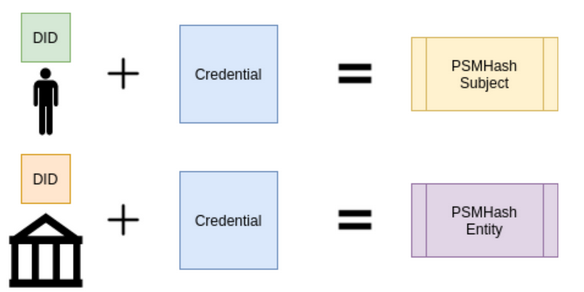
\includegraphics[width=.5\textwidth]{psmhash-credential.png}\hfill
                    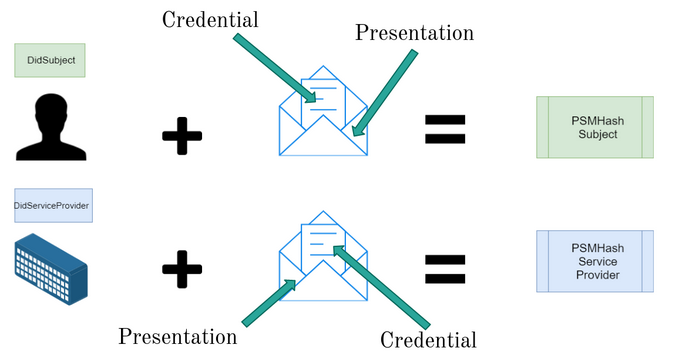
\includegraphics[width=.5\textwidth]{psmhash-presentation.png}
                    \caption{\acrshort{psmh} schema for Credentials and Presentations}
                    \label{fig:psmh}
                \end{figure}
                
                With the \acrshort{psmh} is guaranteed that only the parties involved can "understand" those hashes when they are issued on the blockchain, since it is not the Credential or Presentation itself (the \acrshort{jwt}s) that is transacted on the blockchain, but their \acrshort{psmh}es.
  
            \paragraph{Status of Credentials and Presentations}
                As explained in the previous paragraph, both the Credentials and the Presentations have two ways of being identified, therefore, each of the \acrshort{psmh} has an associated status in the blockchain.
                
                For \textbf{Credentials}, the possible statuses are:
                \begin{itemize}
                    \item \textbf{"0"} or \textbf{"Valid"}: status the Credential has when issued by an Issuer.
                    \item \textbf{"1"} or \textbf{"AskIssuer"}: this status implies that the Issuer of the Credential wants to be asked what the real status of that Credential is.
                    \item \textbf{"2"} or \textbf{"Revoked}: status of the Credential when the issuer revokes it for any reason.
                    \item \textbf{"3"} or \textbf{"DeletedBySubject"}: status when the Subject has removed the Credential.
                \end{itemize}
                
                Similarly, \textbf{Presentations} have the following statuses:
                \begin{itemize}
                  \item \textbf{"0"} or \textbf{"Valid"}: status the Presentation has when issued by a Subject.
                  \item \textbf{"1"} or \textbf{"Received"}: status that the Presentation gets when it is received by a Service Provider.
                  \item \textbf{"2"} or \textbf{"AskDeletion"}: status that the Subject puts when he wants the Presentation to be eliminated and therefore the Credentials that it contains are not used.
                  \item \textbf{"3"} or \textbf{"DeletionConfirmation"}: status that the Service Provider puts in the Presentation when confirming the deletion requested by the Subject previously.
                \end{itemize}
            
    \subsection{Example: Renting a car}
        In this section, an Alastria ID use case will be explained, which is the example that has been carried out in \acrshort{mvp}1\cite{mvp1-car}.\\
        
        In this example, a user (Subject) wants to rent a car, for this, the rental company (Service Provider) asks the user through a Presentation Request for three data: 1) the driving license, 2) his credit card and 3) prove that the user is over 25 years old. 
        \begin{figure}[h]
            \centering
            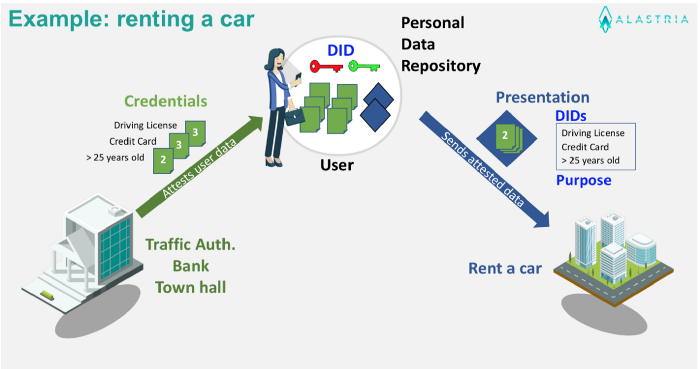
\includegraphics[width=0.8\textwidth]{ala-rent-car.png}
            \caption{Renting a car with Alastria ID}
            \label{fig:ex-car}
        \end{figure}
        The user must send this information to the rental company, and for this he uses Alastria ID and asks the Issuers at that time to certify that the user complies with these conditions. So the user asks the bank for his credit card, asks the traffic authority for his driving license and the town hall to verify he is over 25 years old. Each one of the Issuers (bank, traffic authority and town hall) sends the requested Credentials, and the user stores them in his wallet. The user, having all the needed data in the wallet, creates a Presentation in response to the Presentation Request above. The user sends the Presentation to the rental company. The rental company receives and validates it. Finally, it proceeds to provide the car to the user. All this process can be done directly online without the need for prior registration or verification of the original documents by the rental company. This example can be seen graphically in the figure \ref{fig:ex-car}.\\

        All these information flows between the different actors are registered in the blockchain with different Smart Contracts (figure \ref{fig:rent-cycle}): the Issuer when issuing the Credential calls a Smart Contract to register the issuance, the user (Subject) registers in the blockchain that he has received the same Credential; the user "wraps" the Credentials in a Presentation, indicating why they are delivered and the validity date, signs it and records that he has sent the Presentation; Finally, the Service Provider verifies that the Credentials are valid, consulting the record made by their Issuers, and then records that it has received the Presentation.
        \begin{figure}[h]
            \centering
            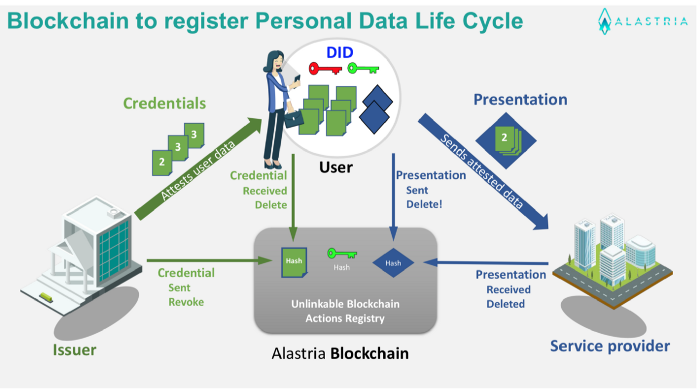
\includegraphics[width=0.8\textwidth]{rent-car-data-lifecycle.png}
            \caption{Alastria ID data life cycle}
            \label{fig:rent-cycle}
        \end{figure}
        
        Registration in the blockchain facilitates the process of checking the validity of the Credentials without the need for direct contact between the rental Service Provider and the Issuers, improving the comfort and privacy of the user (Subject), while reducing the cost and increasing the guarantees for the company.\\

        In addition, registration in the blockchain facilitates the revocation of Credentials by Issuers and the withdrawal (request for deletion) of personal data from users (Subjects).
        
    \subsection{Project structure}
        In this section we will talk about the structure of the first \acrlong{mvp} of Alastria ID (\textit{\acrshort{mvp}1})\cite{ala-mvp1}.\\
        \begin{figure}[h]
            \centering
            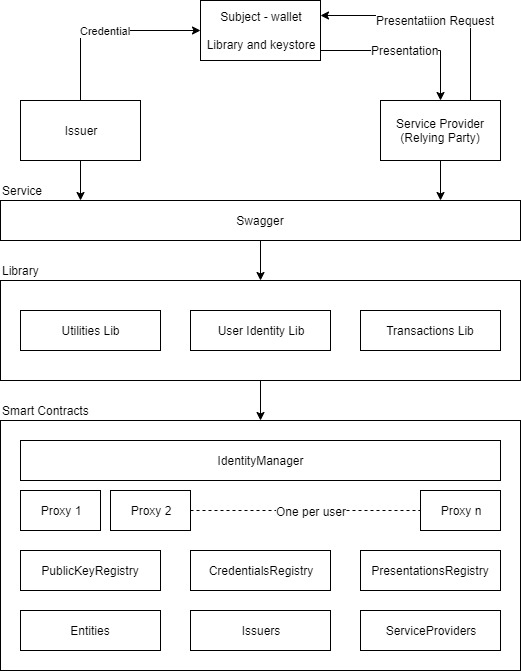
\includegraphics[width=0.7\textwidth]{alastria-mvp1.jpg}
            \caption{Alastria ID MVP1 structure}
            \label{fig:ala_structure}
        \end{figure}
        The \acrshort{mvp}1 is divided into four main parts, as the figure \ref{fig:ala_structure} shows. Although those are not the only parts that are part of the MVP1. There are another series of components that are very important for the ecosystem, such as:
        \begin{itemize}
            \item \textbf{Alastria Node}\footnote{\url{https://github.com/alastria/alastria-node}}: easy documentation and scripts to guide the installation of a blockchain node in the main testnet of Alastria. There are also other guides for different networks, like \textit{Besu}\footnote{\url{https://github.com/alastria/alastria-node-besu}} or \textit{Fabric}\footnote{\url{https://github.com/alastria/alastria-node-fabric}}.
            \item \textbf{Alastria's lib examples}\footnote{\url{https://github.com/alastria/alastria-identity-example}}: use case files to show how to interact with the TypeScript library. This repository is divided according to the different use case that can be done with Alastria ID. There are examples for: creating tokens, creating identities (\acrshort{did}s), creating entities, creating issuers and service providers, creating and deleting credentials and presentations, authentication with Alastria ID, etc.
            \item \textbf{Alastria's objects verification}\footnote{\url{https://github.com/alastria/alastria-identity-JSON-objects}}: this project validates \acrshort{json} objects to see that they are following the specification proposed by Alastria.
        \end{itemize}
        There are still many repositories to mention, which are somehow auxiliary, or are still work in progress.
        
        \subsubsection{Smart Contracts}
            Smart Contracts are the core part of the project, since everything is based on blockchain.\\
            
            It should be mentioned that these Contracts are those created in the first phase of the project (\acrshort{mvp}1). They are not definitive since they have some weaknesses, such as that role governance is not well defined, and they are not Upgradable Smart Contracts.\\
            
            The Smart Contracts are distributed as follows:
            \begin{itemize}
                \item \textbf{Identity Smart Contracts}: this set of Smart Contracts are responsible for generating \acrshort{did}s, managing the different roles of the model (Issuers, Service Providers and Subjects) and making calls between the other Contracts to achieve the correct functioning of the implementation.
                \begin{itemize}
                    \item \textbf{"AlastriaIdentityManager.sol"}\footnote{\url{https://github.com/alastria/alastria-identity/blob/master/contracts/identityManager/AlastriaIdentityManager.sol}}: this is the main Contract, in charge of creating and managing identities. Contracts \textit{"AlastriaIdentityIssuer.sol"} and \textit{"AlastriaIdentityServiceProvider.sol"} assign roles, and this one creates the identities (\acrshort{did}s). This is the only Contract that is deployed, since it inherits the rest of the "identity" Contracts and is in charge of deploying the "registry" Contracts (figure \ref{fig:mvp1-contracts}).
                    \begin{figure}[h]
                        \centering
                        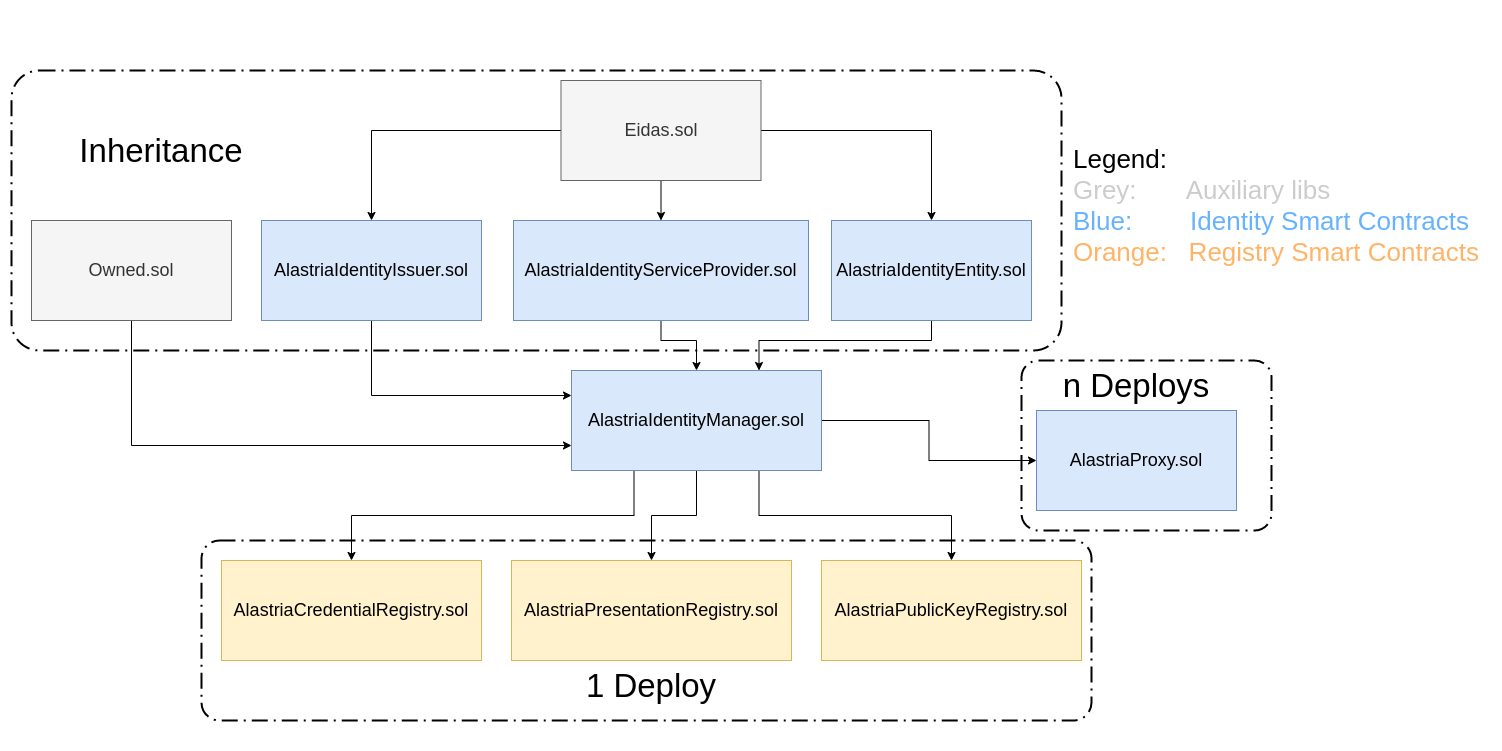
\includegraphics[width=1.0\textwidth]{SCs-Diagram.png}
                        \caption{Alastria ID MVP1 Smart Contracts diagram}
                        \label{fig:mvp1-contracts}
                    \end{figure}
                    \item \textbf{"AlastriaIdentityIssuer.sol"}\footnote{\url{https://github.com/alastria/alastria-identity/blob/master/contracts/identityManager/AlastriaIdentityIssuer.sol}}: this Smart Contract is used to endow the entity with the ability to create identities (\acrshort{did}s) and issue Credentials within the blockchain (remember that we are talking about \acrshort{psmh}es, not \acrshort{jwt}s). To do this, the entity is simply saved in a mapping of issuers and the \acrshort{loa} level, using the library \textit{Eidas.sol}.
                    \item \textbf{"AlastriaIdentityServiceProvider.sol"}\footnote{\url{https://github.com/alastria/alastria-identity/blob/master/contracts/identityManager/AlastriaIdentityServiceProvider.sol}}: similar to the previous Smart Contract, its functionality is to provide the entities with the role of Service Provider. To do this, it stores the entities in a mapping.
                    \item \textbf{"AlastriaIdentityEntity.sol"}\footnote{\url{https://github.com/alastria/alastria-identity/blob/master/contracts/identityManager/AlastriaIdentityEntity.sol}}: it stores entity information, such as name, cif, logo \acrshort{url}, \acrshort{did}, \acrshort{url} of the Alastria Open Access and a flag to know if the entity is active or not.
                    \item \textbf{"AlastriaProxy.sol"}\footnote{\url{https://github.com/alastria/alastria-identity/blob/master/contracts/identityManager/AlastriaProxy.sol}}: this Contract, as its name indicates, acts as a proxy for the account \acrshort{eoa} that is carrying out the transaction. Since any call (except for a few) will always go through the account's proxy. It is responsible for emitting an event of what is being used.
                \end{itemize}
                \item \textbf{Registry Smart Contracts}: these are in charge of managing the Credentials and the Presentations with their respective statuses, also it manages the public keys of the different \acrshort{did}s.
                \begin{itemize}
                    \item \textbf{"AlastriaCredentialRegistry.sol"}\footnote{\url{https://github.com/alastria/alastria-identity/blob/master/contracts/registry/AlastriaCredentialRegistry.sol}}: it is responsible for managing and modifying the different \acrshort{psmh}es of the Credentials through the different statuses. It should be mentioned that a Credential cannot transits to a "lower" or previous status.
                    \item \textbf{"AlastriaPresentationRegistry.sol"}\footnote{\url{https://github.com/alastria/alastria-identity/blob/master/contracts/registry/AlastriaPresentationRegistry.sol}} : this smart contract is analogous to the \textit{"AlastriaCredentialRegistry.sol"} but with the Presentations. Neither the Presentation can transits to a "lower" or previous status.
                    \item \textbf{"AlastriaPublicKeyRegistry.sol"}\footnote{\url{https://github.com/alastria/alastria-identity/blob/master/contracts/registry/AlastriaPublicKeyRegistry.sol}}: stores the public keys of the different identities on the network. It has functionalities to add, modify, delete and verify the public keys.
                \end{itemize}
                \item \textbf{Auxiliary libraries}: standard Smart Contracts designed as libraries that are used to facilitate certain actions or improve functionalities of the previous Smart Contracts.
                \begin{itemize}
                    \item \textbf{"Eidas.sol"}\footnote{\url{https://github.com/alastria/alastria-identity/blob/master/contracts/libs/Eidas.sol}}: Smart Contract created to comply with the regulations of \acrfull{eidas}.
                    \item \textbf{"Owned.sol"}\footnote{\url{https://github.com/alastria/alastria-identity/blob/master/contracts/libs/Owned.sol}}: This is a standard that OpenZeppelin\cite{openzeppelin} has developed that simplifies authorization and control of access to different functions that are implemented in the Smart Contracts.
                \end{itemize}
            \end{itemize}
        
        \subsubsection{TypeScript Library}
            This library\footnote{\url{https://github.com/alastria/alastria-identity-lib}} written in \textit{TypeScript} has been created to facilitate interaction with Smart Contracts previously mentioned.\\
            
            This library has three different modules:
            \begin{itemize}
                \item \textbf{User functions}: it helps to manage the wallet and the identity user. Also helps when signing transactions.
                \item \textbf{Blockchain functions}: it encapsulates the Alastria ID Smart Contracts, so that only functions have to be called with TypeScript, without needing to know how to write in Solidity in order to work with the Smart Contracts. This module is divided as are the Smart Contracts. So, for example, the \textit{"AlastriaPublicKeyRegistry.sol"} can be found in the file \textit{"publicKeyRegistryTransactionFactory.ts"}\footnote{\url{https://github.com/alastria/alastria-identity-lib/blob/master/src/txFactory/publicKeyRegistryTransactionFactory.ts}}. It is the same for the rest of the main Smart Contracts.
                \item \textbf{Tokens functions}: it manages the different \acrshort{jwt}s explained previously, guaranteeing that they are well built and are valid. It also allows the signing and decoding of said \acrshort{jwt}s.
            \end{itemize}
            
        \subsubsection{Wallet}
            The Alastria ID wallet\footnote{\url{https://github.com/alastria/alastria-wallet}}, is a mobile application written in \textit{Ionic} to implement the different user stories of Alastria ID. This wallet is a \acrfull{poc}, which means it is not a valid wallet for a project in production. This is because it does many things in a "fake way" since the objective was not to be a commercial product.\\
            
            In the secure part of the wallet (called \textit{secure storage}) the keys are generated and stored that users use to sign and verify such signatures. Herein lies one of the main problems of this wallet, since it is not a \textit{multidivice wallet}, that is, each pair of keys is only and only for one device (wallet). Another of the main problems is that the key recovery or modification flow has not yet been defined, so if the wallet is removed from the device, the identity would be lost.\\
            
            To finish this section, we will explain what and how are the keys that are stored in the wallet are. This keys are called \textit{keystores}. This \textit{keystores} is nothing other than an \acrfull{eoa} used to interact with the blockchain. The listing \ref{lst:keystore} shows an example of a \textit{keystore}.
            \lstinputlisting[language=json,label={lst:keystore}, caption=Keystore example]{examples/codeSnippets/keystore.json}
        
        \subsubsection{Entity}
            It is called "Entity" to an example implementation to simulate an entity\footnote{\url{https://github.com/alastria/alastria-identity-entity}}. This entity has both roles, Issuer and Service Provider. It is designed to interact with the wallet to perform the full \acrshort{poc} for the \acrshort{mvp}1. It contains a \textit{Mongo} database that is used to store certain information.\\
            
            This implementation is divided into two parts: the backend and the frontend.
            \begin{itemize}
                \item \textbf{Backend}: written with \textit{Swagger} and \textit{NodeJS} and it is in charge of interacting with the Smart Contracts, making use of the previously mentioned \textit{TypeScript} library. The following operations can be performed: create an identity (\acrshort{did}), issue Credentials and receive Presentations, as well as check the statuses of both. It stores and reads information in the database.
                \item \textbf{Frontend}: developed with \textit{Angular}, \textit{JavaScript} and \textit{Nginx}. It is the facade to interact with the backend and offer a better user experience than by using scripts. Currently it can be checked online\footnote{As it is a temporary demo, it may no longer be operational \url{http://34.244.47.233/login}}.
            \end{itemize}
\newpage
\section{Security audit}
    In this section a security audit of the Smart Contracts and the \textit{TypeScript} library will be performed. Various tools will be used and the vulnerabilities found will be listed along with their level of criticality.
    
    \subsection{Audit of the Smart Contracts}
        The objective of this subsection is to perform a security analysis of the Smart Contracts from the  \acrshort{mvp}1 in order to detect vulnerabilities, with the aim of improving the quality of the Contracts.\\
        
        For this purpose, two analyses will be made. One with the tool \textit{Mythril}\footnote{\url{https://github.com/ConsenSys/mythril}}. \textit{Mythril} (figure \ref{fig:myth}) is a security analysis tool for \acrshort{evm} bytecode. It detects security vulnerabilities in Smart Contracts built for \textit{Ethereum}, \textit{Hedera}, \textit{Quorum}, \textit{Vechain}, \textit{Roostock}, \textit{Tron} and other \acrshort{evm}-compatible blockchains. It uses symbolic execution, \acrshort{smt} solving and taint analysis to detect a variety of security vulnerabilities.
        \begin{figure}[h]
            \centering
            
\includegraphics[width=0.3\textwidth]{mythril_logo.png}
            \caption{Mythril logo}
            \label{fig:myth}
        \end{figure}
        
        In addition, a dead code analysis will be done, to detect failures in the code of the Smart Contracts.
        
        \subsubsection{Mythril analysis}
            In the \acrshort{mvp}1 of Alastria ID, eight Smart Contracts have been designed and two libraries have been used.\\
            
            To facilitate the audit, some scripts have been designed in \textit{Shell Script}. The first script called \textit{audit.sh} (listing \ref{lst:audit.sh}) performs the analysis with the \textit{Mythril} tool. A docker container has been created for each contract and the analysis has been carried out in this container. This analysis has been programmed to last a maximum of two hours.
        
            \lstinputlisting[label={lst:audit.sh}, caption=audit.sh source code, language=bash]{examples/mythrilAudit/audit.sh}
        
            In order to obtain the reports after the completion of \textit{audit.sh}, another script has been made, called \textit{getReports.sh} (listing \ref{lst:getReports.sh}). This script copies the logs of the different containers created into different files, so that they are more comfortable to handle and read.\\
            
            \lstinputlisting[label={lst:getReports.sh}, caption=getReports.sh source code, language=bash]{examples/mythrilAudit/getReports.sh}
            
            After the analysis, and the study of the reports, the following results have been obtained:
            \paragraph{AlastriaCredentialRegistry.sol}
                The following table (table \ref{tab:AlastriaCredentialRegistry}) summarizes the vulnerabilities found in the Smart Contract \textit{AlastriaCredentialRegistry}.
                \begin{longtable}{||p{0.1\linewidth} | p{0.11\linewidth} | p{0.52\linewidth} | p{0.3\linewidth}||}
                    \hline
                    \textbf{\acrshort{swc} ID} & \textbf{Severity} & \textbf{Functions} & \textbf{Description} \\ [0.5ex] 
                    \hline\hline
                    \href{https://swcregistry.io/docs/SWC-101}{101} & High & addSubjectCredential (bytes32, string) & The arithmetic operator can overflow.\\ 
                    \hline
                    \href{https://swcregistry.io/docs/SWC-110}{110} & Medium & issuerCredentialList (address, uint256) & An assertion violation was triggered.\\
                    \cline{3-3}
                    & & getCredentialStatus (uint8, uint8) &\\ 
                    \cline{3-3} 
                    & & subjectCredentialList (address, uint256) &\\
                    \cline{3-3}
                    & & updateCredentialStatus (bytes32, uint8) &\\ [1ex] 
                    \hline
                    \caption{AlastriaCredentialRegistry.sol Mythrill audit report}
                    \label{tab:AlastriaCredentialRegistry}
                \end{longtable}

            \newpage

            \paragraph{AlastriaIdentityEntity.sol}
                The following table (table \ref{tab:AlastriaIdentityEntity}) summarizes the vulnerabilities found in the Smart Contract \textit{AlastriaIdentityEntity}.
                \begin{longtable}{||p{0.1\linewidth} | p{0.11\linewidth} | p{0.5\linewidth} | p{0.3\linewidth}||}
                    \hline
                    \textbf{\acrshort{swc} ID} & \textbf{Severity} & \textbf{Functions} & \textbf{Description} \\ [0.5ex] 
                    \hline\hline
                    \href{https://swcregistry.io/docs/SWC-101}{101} & High & setUrlLogo (address, string) & The arithmetic operator can overflow. \\
                    \cline{3-3}
                    & & setCifEntity (address, string)  &\\
                    \cline{3-3}
                    & & setUrlCreateAID (address, string) &\\
                    \cline{3-3}
                    & & setUrlAOA (address, string) &\\
                    \cline{3-3}
                    & & setNameEntity (address, string) &\\[1ex] 
                    \hline
                    \caption{AlastriaIdentityEntity.sol Mythrill audit report}
                    \label{tab:AlastriaIdentityEntity}
                \end{longtable}
                
            \paragraph{AlastriaIdentityIssuer.sol}
                The following table (table \ref{tab:AlastriaIdentityIssuer}) summarizes the vulnerabilities found in the Smart Contract \textit{AlastriaIdentityIssuer}.
                \begin{longtable}{||p{0.1\linewidth} | p{0.11\linewidth} | p{0.45\linewidth} | p{0.35\linewidth}||}
                    \hline
                    \textbf{\acrshort{swc} ID} & \textbf{Severity} & \textbf{Functions} & \textbf{Description} \\ [0.5ex] 
                    \hline\hline
                    \href{https://swcregistry.io/docs/SWC-107}{107} & Low & updateIdentityIssuerEidasLevel\newline (address, uint8) & Read of persistent state following external call.\\
                    \cline{3-3}
                    & & addIdentityIssuer (address, uint8) &\\[1ex]
                    \hline
                    \href{https://swcregistry.io/docs/SWC-110}{110} & Medium & updateIdentityIssuerEidasLevel\newline (address, uint8) & An assertion violation was triggered.\\
                    \cline{3-3}
                    & & addIdentityIssuer (address, uint8) &\\
                    \cline{3-3}
                    \hline
                    \caption{AlastriaIdentityIssuer.sol Mythrill audit report}
                    \label{tab:AlastriaIdentityIssuer}
                \end{longtable}
                
            \paragraph{AlastriaIdentityManager.sol}
                No vulnerabilities were found in \textit{AlastriaIdentityManager.sol} after the audit.
                
            \paragraph{AlastriaIdentityServiceProvider.sol}
                No vulnerabilities were found in \textit{AlastriaIdentityServiceProvider.sol} after the audit.
                
            \paragraph{AlastriaPresentationRegistry.sol}
                No vulnerabilities were found in \textit{AlastriaPresentationRegistry.sol} after the audit.
                
            \paragraph{AlastriaProxy.sol}
                The following table (table \ref{tab:AlastriaProxy}) summarizes the vulnerabilities found in the Smart Contract \textit{AlastriaIdentityIssuer}.\newline
                \begin{longtable}{||p{0.1\linewidth} | p{0.11\linewidth} | p{0.45\linewidth} | p{0.35\linewidth}||}
                    \hline
                    \textbf{\acrshort{swc} ID} & \textbf{Severity} & \textbf{Functions} & \textbf{Description} \\ [0.5ex] 
                    \hline\hline
                    \href{https://swcregistry.io/docs/SWC-107}{107} & Low & forward (address, uint256, bytes) & A call to a user-supplied address is executed. An external message call to an address specified by the caller is executed.\\ [1ex] 
                    \hline
                    \caption{AlastriaProxy.sol Mythrill audit report}
                    \label{tab:AlastriaProxy}
                \end{longtable}
                
            \paragraph{AlastriaPublicKeyRegistry.sol}
                The following table (table \ref{tab:AlastriaPublicKeyRegistry}) summarizes the vulnerabilities found in the Smart Contract \textit{AlastriaPublicKeyRegistry}.
                \begin{longtable}{||p{0.1\linewidth} | p{0.11\linewidth} | p{0.45\linewidth} | p{0.35\linewidth}||}
                    \hline
                    \textbf{\acrshort{swc} ID} & \textbf{Severity} & \textbf{Functions} & \textbf{Description} \\ [0.5ex] 
                    \hline\hline
                    \href{https://swcregistry.io/docs/SWC-110}{110} & Medium & publicKeyList (address, uint256) & An assertion violation was triggered.\\ [1ex] 
                    \hline
                    \caption{AlastriaPublicKeyRegistry.sol Mythrill audit report}
                    \label{tab:AlastriaPublicKeyRegistry}
                \end{longtable}
        
            \paragraph{Eidas.sol}
                The following table (table \ref{tab:Eidas}) summarizes the vulnerabilities found in the Smart Contract \textit{Eidas}.
                \begin{longtable}{||p{0.1\linewidth} | p{0.11\linewidth} | p{0.50\linewidth} | p{0.30\linewidth}||}
                    \hline
                    \textbf{\acrshort{swc} ID} & \textbf{Severity} & \textbf{Functions} & \textbf{Description} \\ [0.5ex] 
                    \hline\hline
                    \href{https://swcregistry.io/docs/SWC-110}{110} & Medium & atLeast\newline (Eidas.EidasLevel, Eidas.EidasLevel) & An assertion violation was triggered.\\
                    \cline{3-3}
                    & & atLeastLow (Eidas.EidasLevel) &\\[1ex] 
                    \hline
                    \caption{Eidas.sol Mythrill audit report}
                    \label{tab:Eidas}
                \end{longtable}
                
            \paragraph{Owned.sol}
                No vulnerabilities were found in \textit{Owned.sol} after the audit.\\

            \begin{figure}[h]
                \centering
                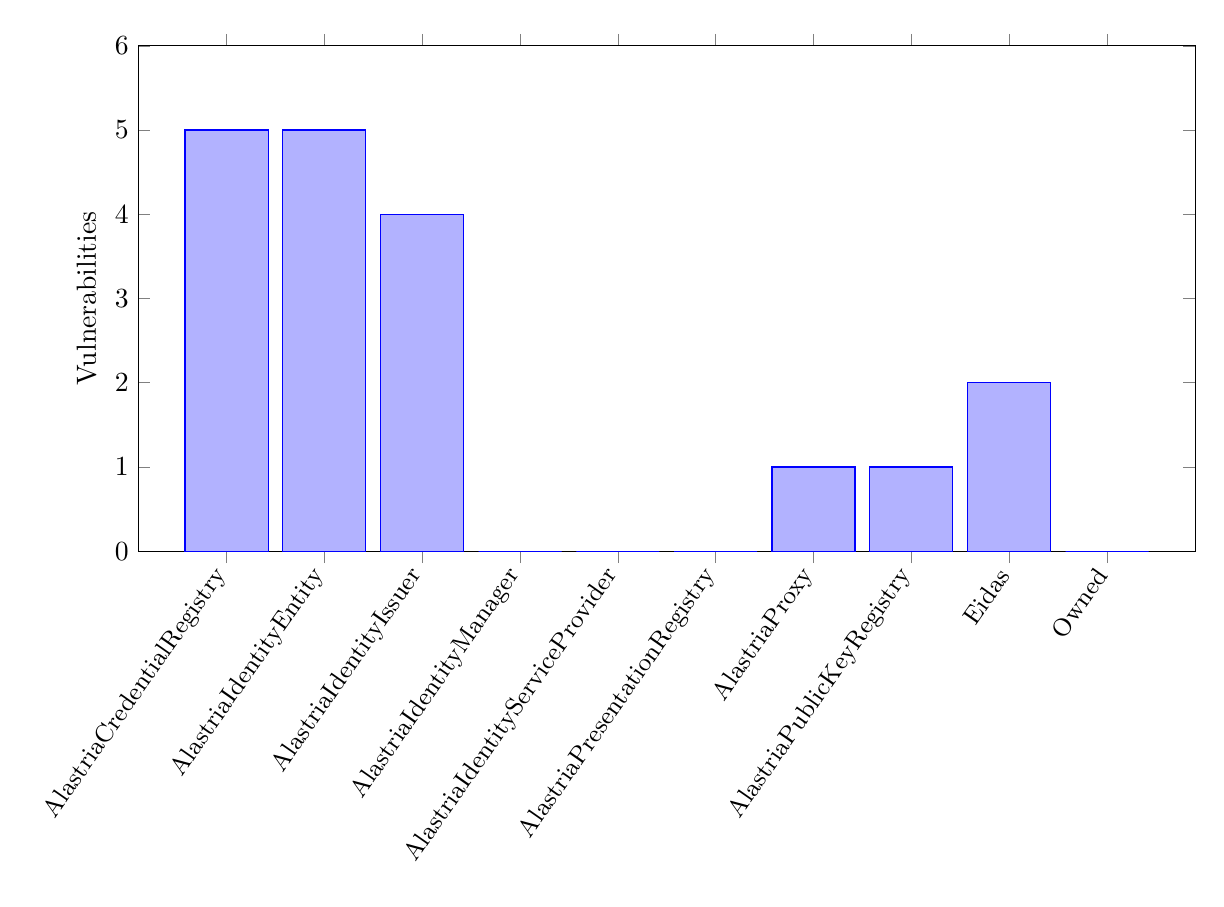
\begin{tikzpicture}
                    \begin{axis}[
                     width=15cm,
                     height=8cm,
                     symbolic x coords={AlastriaCredentialRegistry, AlastriaIdentityEntity, AlastriaIdentityIssuer, AlastriaIdentityManager, AlastriaIdentityServiceProvider, AlastriaPresentationRegistry, AlastriaProxy, AlastriaPublicKeyRegistry, Eidas, Owned},
                     x tick label style={rotate=55, font=\small,anchor=east},
                     xtick=data,
                     ymin=0,
                     ymax=6,
                     ylabel=Vulnerabilities,
                     ybar,
                     bar width=30pt,
                     ]
                    \addplot coordinates {
                        (AlastriaCredentialRegistry, 5)
                        (AlastriaIdentityEntity, 5)
                        (AlastriaIdentityIssuer, 4)
                        (AlastriaIdentityManager, 0)
                        (AlastriaIdentityServiceProvider, 0)
                        (AlastriaPresentationRegistry, 0)
                        (AlastriaProxy, 1)
                        (AlastriaPublicKeyRegistry, 1)
                        (Eidas, 2)
                        (Owned, 0)};
                    \end{axis}
                \end{tikzpicture}
                \caption{Number of vulnerabilities by Smart Contract}
                \label{fig:bars-scs}
            \end{figure}
            
            In conclusion to the analysis, we can see that Smart Contracts \textit{AlastriaCredentialRegistry} and \textit{AlastriaIdentityEntity} are the ones that have found the most vulnerabilities, with five each one (figure \ref{fig:bars-scs}). In relation to the vulnerabilities found, we see that \textbf{33\% (6) are high}, another \textbf{55\% (9) are medium} and \textbf{17\% (3) are low} (figure \ref{fig:pie-scs}).\\
            \begin{figure}[h!]
                \centering
                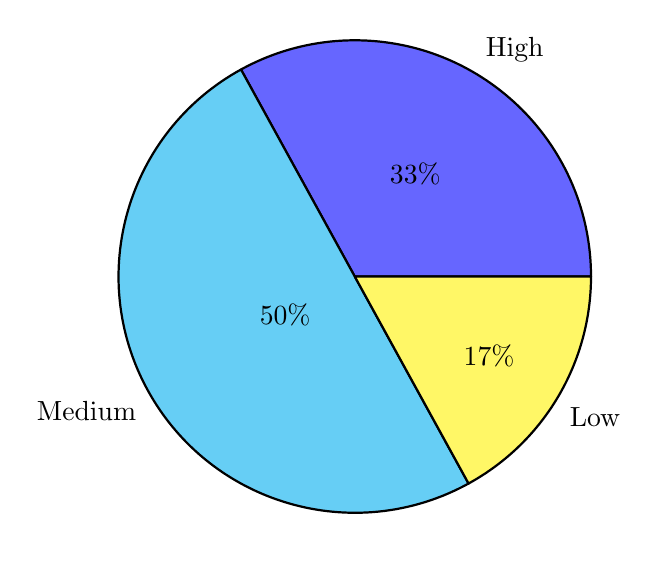
\begin{tikzpicture}
                    \pie{33/High, 50/Medium, 17/Low}
                \end{tikzpicture}
                \caption{Criticality of the Smart Contracts vulnerabilities}
                \label{fig:pie-scs}
            \end{figure}
        
            Below are some points to mitigate the vulnerabilities found.\\
            
            An \textbf{arithmetic overflow (\acrshort{swc} \href{https://swcregistry.io/docs/SWC-101}{101})} means that it is possible to cause an integer overflow or underflow in an arithmetic operation. This means that you can store in a variable a value larger than its limit. This can be solved by checking if it is possible to overflow or underflow before performing the operation. It is advisable to use standard libraries already defined that mitigate this attack. An example of a standard library is \textit{SafeMath.sol}\footnote{\url{https://github.com/OpenZeppelin/openzeppelin-contracts/blob/master/contracts/math/SafeMath.sol}}, developed by \textit{OpenZeppelin}.\\
            
            In relation to the \textbf{reentrancy (\acrshort{swc} \href{https://swcregistry.io/docs/SWC-107}{107})}, an external message call to an address specified by the caller can be executed. The callee account might contain arbitrary code and could re-enter any function within this contract. Reentering the contract in an intermediate state may lead to unexpected behavior. To mitigate this, you have t make sure that no state modifications are executed after the call and/or reentrancy guards are in place. Also, with this vulnerability, the contract account state is accessed after an external call to a fixed address. To prevent reentrancy issues, consider accessing the state only before the call, especially if the callee is untrusted. Alternatively, a reentrancy lock can be used to prevent untrusted callees from re-entering the contract in an intermediate state.\\
            
            Finally, about the \textbf{assert violation (\acrshort{swc} \href{https://swcregistry.io/docs/SWC-110}{110})}, \textit{Solidity} \textit{assert()} statements should only be used to check invariants. Review the transaction trace generated for this issue and either make sure your program logic is correct, or use \textit{require()} instead of \textit{assert()} if your goal is to constrain user inputs or enforce preconditions. Remember to validate inputs from both callers (for instance, via passed arguments) and callees (for instance, via return values).

        
        \subsubsection{Dead code analysis}
            In this part of the audit, no tools have been used. The objective of this analysis has been to read the contracts carefully and, having understood and assimilated the Alastria ID model, to detect programming errors, requirements errors or functional errors that differ from the theoretical implementation of the model.\\
            
            After a detailed study, and without entering into design analysis (the quality of code, structure of the project or naming of functions and variables has not been evaluated), a vulnerability has been detected regarding the permissions of who can call which function. This is summarized in the following table (table \ref{tab:dead-code-issuer}):
            \begin{longtable}{||p{0.5\linewidth} | p{0.5\linewidth}||}
                \hline
                \textbf{Function}  & \textbf{Modifiers}\\ [0.5ex] 
                \hline\hline
                updateIdentityIssuerEidasLevel\newline (address \_identityIssuer,\newline Eidas.EidasLevel \_level) & alLeastLow (\_level)\newline onlyIdentityIssuer (\_identityIssuer)\\ 
                \hline
                deleteIdentityIssuer\newline (address \_identityIssuer) & onlyIdentityIssuer (\_identityIssuer)\\[1ex] 
                \hline
                \caption{AlastriaIdentityIssuer.sol dead code analysis}
                \label{tab:dead-code-issuer}
            \end{longtable}
            The vulnerability lies in the fact that a misuse of modifiers is being made.  In the two functions listed, the modifier \textit{"onlyIdentityIssuer (\_identityIssuer)"} is used. That modifier evaluates whether or not the input argument \textit{(\_identityIssuer)} is an Issuer. The error is that the modifier's argument \textit{(\_identityIssuer)} is the same as the function's input argument, when the model want to evaluate if the \textit{msg.sender} (the one who calls the function) is or is not an Issuer.\\
            
            Bearing in mind that the role of Issuer is that which allows you to create identities (\acrshort{did}s), this vulnerability has been classified as "high" (8.9 overall score) and the following attack vector has been calculated\footnote{The detailed score can be checked \href{https://nvd.nist.gov/vuln-metrics/cvss/v3-calculator?vector=AV:N/AC:L/PR:H/UI:N/S:C/C:N/I:H/A:H/E:F/RL:O/RC:R/CR:X/IR:H/AR:H/MAV:N/MAC:L/MPR:N/MUI:N/MS:C/MC:X/MI:H/MA:H&version=3.1}{here}} (figure \ref{fig:stats-aii}).\\
            \begin{figure}[h]
                \centering
                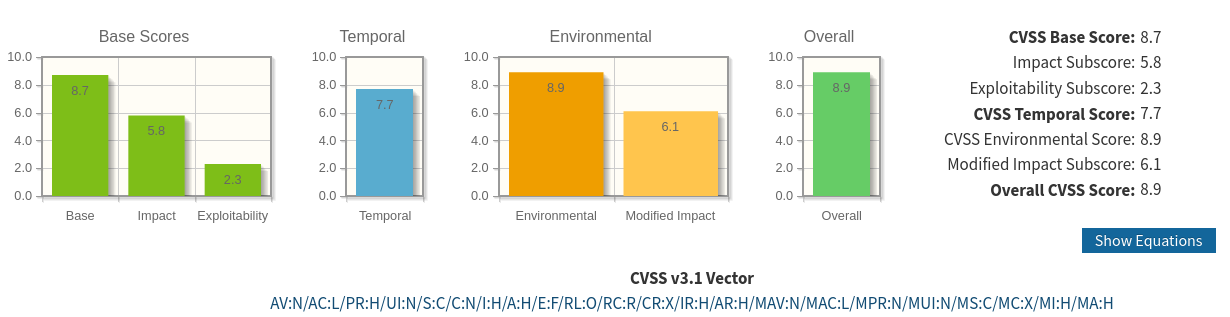
\includegraphics[width=1.1\textwidth]{stats-aii.png}
                \caption{\acrshort{cvss} stats for AlastriaIdentityIssuer.sol}
                \label{fig:stats-aii}
            \end{figure}
            
            With the intention of visualizing and understanding the criticality of this vulnerability, later in the document a \acrfull{poc} will be done, more specifically, exploiting the function "\textit{deleteIdentityIssuer}".\\
            
            Something similar happens with the Smart Contract AlastriaIdentityEntity (table \ref{tab:dead-code-entity}):
            
            \begin{longtable}{||p{0.5\linewidth} | p{0.5\linewidth}||}
                \hline
                \textbf{Function}  & \textbf{Modifiers}\\ [0.5ex] 
                \hline\hline
                setNameEntity\newline (address \_addressEntity, string \_name) & onlyIdentityEntity (\_addressEntity)\\
                \hline
                setCifEntity\newline (address \_addressEntity,\newline string \_cif) & onlyIdentityEntity (\_addressEntity)\\
                \hline
                setUrlLogo\newline (address \_addressEntity,\newline string \_url\_logo) & onlyIdentityEntity (\_addressEntity)\\
                \hline
                setUrlCreateAID\newline (address \_addressEntity,\newline string \_url\_createAID) & onlyIdentityEntity (\_addressEntity)\\
                \hline
                setUrlAOA\newline (address \_addressEntity,\newline string \_url\_AOA)  & onlyIdentityIssuer (\_identityIssuer)\\[1ex] 
                \hline
                \caption{AlastriaIdentityEntity.sol dead code analysis}
                \label{tab:dead-code-entity}
            \end{longtable}
            The same error occurs as the one mentioned above. The modifier \textit{"onlyIdentityEntity (\_addressEntity)"} must be with \textit{"onlyIdentityEntity (msg.sender)"} instead of the current one.\\
            
            The vulnerability, although it no longer affects the creation of identities (\acrshort{did}s), remains at a "high" level (8.9), but it has a different attack vector\footnote{The detailed score can be checked \href{https://nvd.nist.gov/vuln-metrics/cvss/v3-calculator?vector=AV:N/AC:L/PR:H/UI:N/S:C/C:H/I:N/A:N/E:F/RL:O/RC:R/CR:H/IR:X/AR:X/MAV:N/MAC:L/MPR:N/MUI:N/MS:C/MC:H/MI:X/MA:X&version=3.1}{here}} (figure \ref{fig:stats-aii}).\\
            \begin{figure}[h]
                \centering
                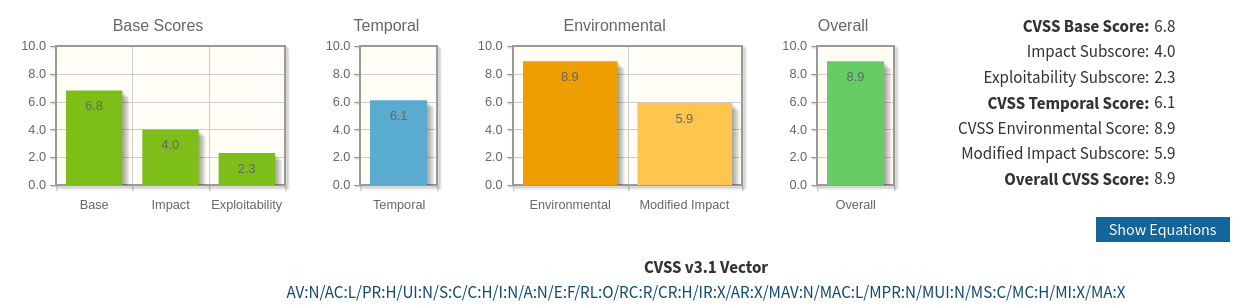
\includegraphics[width=1.1\textwidth]{stats-aie.png}
                \caption{\acrshort{cvss} stats for AlastriaIdentityEntity.sol}
                \label{fig:stats-aie}
            \end{figure}
        \subsection{Audit of the TypeScript Library}
            % TODO
            %2- Lib node
            %objetivo tal
            %HERRAMIENTAS utilzadas (myth y análisis de código muerto)
            %CÓMO LO HE HECHO
            %RESUMEN REPORT (TABLAS Y TEXTO)

\newpage
\section{PoC Attack}
    As mentioned previously, in this section we are going to present a \acrfull{poc} by exploiting a vulnerability found in the section adobe, more specifically the vulnerability found in the dead code analysis, in the function \textit{"deleteIdentityIssuer"}. The \acrshort{poc} agents will be explained, then it will be shown graphically what they should be able to do and what they really can do. Later, the attack flow will be explained and the code written to perform it. Finally, the criticality of the attack will be discussed again, as well as the reasons and consequences of what it would mean to reach production with such a vulnerability.

    \subsection{Agents and permissions}
        In the following figure (figure \ref{fig:poc-actors}) shows the different agents and it's permissions before the \acrshort{poc}.\\ 
        \begin{figure}[h]
            \centering
            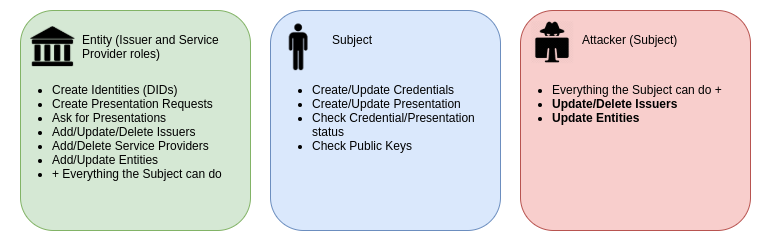
\includegraphics[width=1.0\textwidth]{poc-actors.png}
            \caption{\acrshort{poc} agents and permissions}
            \label{fig:poc-actors}
        \end{figure}
        
        The entity will have the roles of Issuer and Service Provider, but we will only focus on the Issuer role. We will also have an attacker, with the same permissions as a Subject. This means that, the only thing the attacker has is it's own \acrshort{did} (has no more privileges). As we can see, the entity, which can be a bank or a traffic authority, can create Credentials, Presentations, consult public keys and create identities (\acrshort{did}s) among other things. The creation of identities is what interests us in this \acrshort{poc}. We see that the attacker has the ability to delete Issuers, which he should not be able to do. By exploiting this vulnerability, we will stop an entity from being an Issuer, and therefore, from being able to create new identities, as we see graphically in the figure \ref{fig:poc-actors-after}.
        
        \begin{figure}[h]
            \centering
            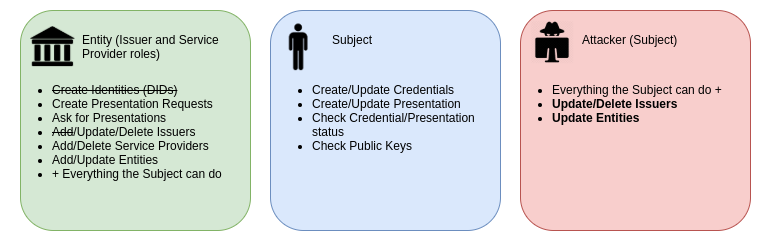
\includegraphics[width=1.1\textwidth]{poc-actors-after.png}
            \caption{\acrshort{poc} agents and permissions after de attack}
            \label{fig:poc-actors-after}
        \end{figure}
    
    \subsection{Attack flow}
        The figure \ref{fig:poc-flow} shows the flow that will be followed to carry out this attack.
        \begin{figure}[h]
            \centering
            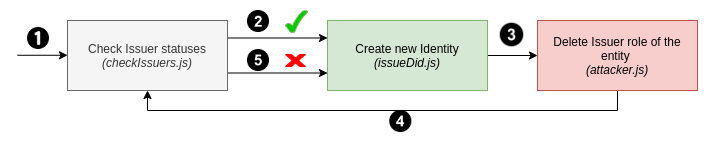
\includegraphics[width=1.1\textwidth]{poc-flow.png}
            \caption{Attack flow}
            \label{fig:poc-flow}
        \end{figure}
        
        The \acrshort{poc} consists of five parts. First, a script written in \textit{NodeJS} (listing \ref{lst:checkIssuers.js}) has been created, which checks whether the entity and the attacker have the role of Issuer. In the first step (1) it will check that the entity is an Issuer, but the attacker is not.\\
        \lstinputlisting[label={lst:checkIssuers.js}, caption=checkIssuers.js source code, language=ES6]{examples/poc/checkIssuers.js}
        
        Then it will be tested that the entity can correctly create new identities (2), for this we will use the script, also written in \textit{NodeJS} \textit{"issueDid.js"} (listing \ref{lst:issueDid.js}). After the execution, it will be possible to see the new \acrshort{did} created.\\
        \lstinputlisting[label={lst:issueDid.js}, caption=issueDid.js source code, language=ES6]{examples/poc/issueDid.js}
        
        The third step is the attack itself (3). At this point, the attacker (who we know is not an Issuer) will remove the entity from the Issuers list. Thus getting the entity to stop providing the service of creating identities, which can mean a lack of integrity and availability. This script is also written in \textit{NodeJS} (listing \ref{lst:attacker.js}).\\
        \lstinputlisting[label={lst:attacker.js}, caption=attacker.js source code, language=ES6]{examples/poc/attacker.js}
        
        Having carried out the attack successfully, only the last steps are missing, which basically is to repeat the first two to verify that the entity has stopped being able to provide the service. First we will check if the entity and the attacker are Issuers (4) but we will see that now neither of them has that role. This will be done by running the script \textit{checkIssuers.js} (listing \ref{lst:checkIssuers.js}) again. \\
        
        Finally, we will try to create a new identity (5) with the \textit{issueDid.js} script, but we will not be able to generate a \acrshort{did} this time and checking the inability of the service.\\
        
        To be able to re-establish the service in the entity, we would need a second entity with the role of Issuer, and that would add the first entity as Issuer. But even so, the same problem would still exist, and any malicious Subject (attacker) could carry out the attack again.
        
    \subsection{The attack}
        In this section will follow the order established in the previous section, and will show screenshots of the executions described above. The figure \ref{fig:poc-tree} shows the general structure of this project, with the different files needed (the dependencies generated after \textit{npm install} have been omitted).\\
        \begin{figure}[h]
            \centering
            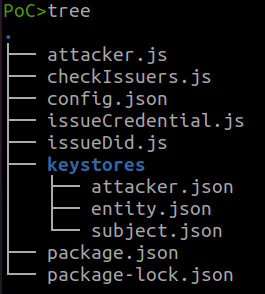
\includegraphics[width=0.4\textwidth]{poc/tree.png}
            \caption{\acrshort{poc} tree}
            \label{fig:poc-tree}
        \end{figure}
        
        As already mentioned, we first visualize the roles of the entity and the attacker (1). The figure \ref{fig:poc-1} shows the output of the \textit{checkIssuers.js} script (listing \ref{lst:checkIssuers.js}). We can easily verify that the entity is an Issuer, but the attacker is not.\\
        \begin{figure}[h]
            \centering
            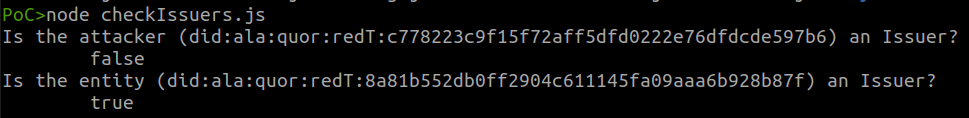
\includegraphics[width=1.0\textwidth]{poc/1.png}
            \caption{checkIssuers.js output before the attack}
            \label{fig:poc-1}
        \end{figure}
        
        Then, from the entity we created a new identity (2) with the help of \textit{issueDid.js} (listing \ref{lst:issueDid.js}). We check that there is no problem when performing the service (figure \ref{fig:poc-2}).\\
        \begin{figure}[h]
            \centering
            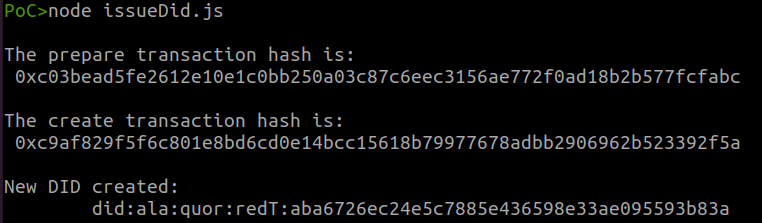
\includegraphics[width=1.0\textwidth]{poc/2.png}
            \caption{issueDid.js output before the attack}
            \label{fig:poc-2}
        \end{figure}
        
        The third step is the attacker's turn (3), where using the \textit{attacker.js} script (listing \ref{lst:attacker.js}). This output (figure \ref{fig:poc-3}) does not provide anything interesting, except the hash of the transaction made.\\
        \begin{figure}[h]
            \centering
            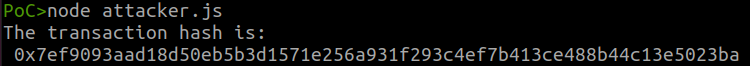
\includegraphics[width=1.0\textwidth]{poc/3.png}
            \caption{attacker.js output}
            \label{fig:poc-3}
        \end{figure}
        
        To verify that the attack has been successful (4), we run the Issuer status check on the entity and the attacker again (figure \ref{fig:poc-4}). This time we see that the entity (\acrshort{did} "did:ala:quor:redT:8a81b552db0ff2904c611145fa09aaa6b928b87f") is not an Issuer.\\
        \begin{figure}[h]
            \centering
            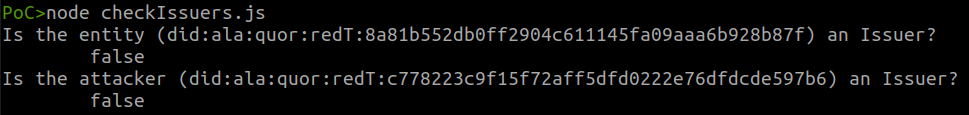
\includegraphics[width=1.0\textwidth]{poc/4.png}
            \caption{checkIssuers.js output after the attack}
            \label{fig:poc-4}
        \end{figure}
        
        The last check that is made, is to try again to create an identity. We run again \textit{issueDid.js} (listing \ref{lst:issueDid.js}), but now in the output (figure \ref{fig:poc-5}) we see an error \textit{"ERROR prepare: Error: Transaction has been reverted by the EVM"}. This error indicates that the \textit{"prepare"} transaction, that is the first one of two that is made for the identity creation, has failed. This is because now the entity does not satisfy the modifier of the function \textit{prepareAlastriaID} of the Smart Contract \textit{AlastriaIdentityManager.sol}\footnote{\url{https://github.com/alastria/alastria-identity/blob/master/contracts/identityManager/AlastriaIdentityManager.sol\#L52}}. The modifier requires that the function caller has the Issuer role.
        \begin{figure}[h]
            \centering
            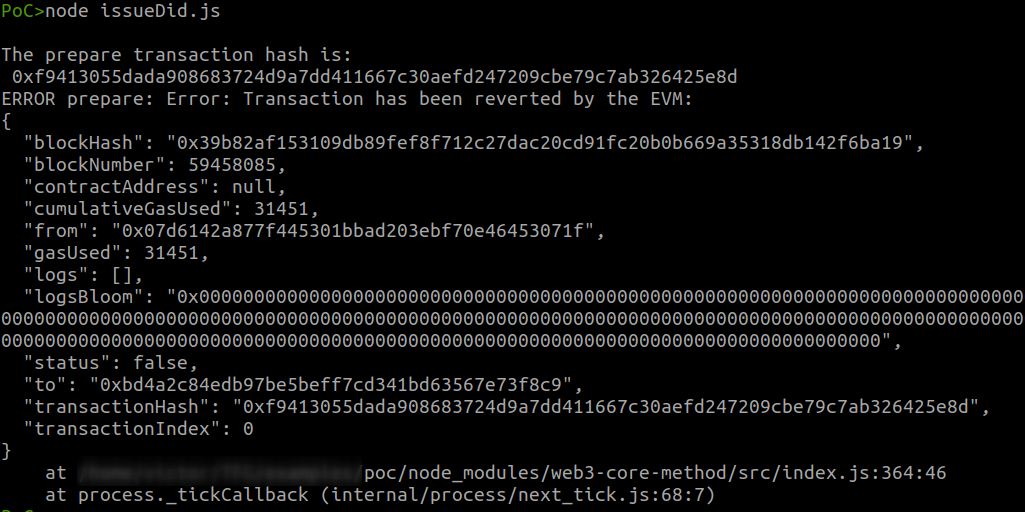
\includegraphics[width=1.0\textwidth]{poc/5.png}
            \caption{issueDid.js output after the attack}
            \label{fig:poc-5}
        \end{figure}
        
    \subsection{Criticity and Impact}
        In section \textit{4.1.2 Dead code analysis}, this vulnerability has been given \acrshort{cvss} score of 8.9 ("high"). This criticality is due to the critical service that the entity performs, such as creating identities (\acrshort{did}s). To give an example, it would be as if a bank (the entity) could not register new users. This loss of service would imply the loss of new clients, which could be a great economic loss for the entity in a real environment.\\

        This vulnerability could also cause concern to the rest of the entities in the blockchain network, since they would find themselves working in an ecosystem that would not be safe.\\
        
        Fortunately, this vulnerability has been found in the \acrshort{mvp}1, and the team in charge of correcting this bug has already been notified. Therefore, it will be corrected in the next phase of the Alastria ID model.\\
        
        After the study carried out in this thesis, a series of improvements to the model, that are not within the scope of this thesis, have also been found. This improvements have already been notified and are being treated in the different Alastria working groups, such as the quality and structure of the code and the governance of roles, that in the next version of Alastria ID will improve.
        
\newpage
\section{Conclusions}
% TODO hacer

\newpage
\section{Future Work}
% TODO hacer
%si vamos bien
%3- entity
%si voy sobrado
%4 - wallet
\newpage
% \nocite{*} % Cita todas las ref (incluidas las no citadas)
\printbibliography[heading=bibnumbered] % Última sección, numerada, para la bibliografía

\end{document}

